% !TeX root = ../documento.tex
\chapter{Metodologia específica: controle do sistema hidraulico nao linear}
\label{cap:controle}

Neste capítulo apresenta-se a metodologia específica adotada para o projeto e a avaliação de uma estratégia de controle digital aplicada ao sistema de freio, com foco na implementação de estratégias de frenagem ativa baseadas em modulação de pressão. A partir dessa estratégia, torna-se possível ajustar a força de frenagem de forma automatizada, viabilizando, entre outras aplicações, o atendimento a referências de desaceleração provenientes de sistemas de assistência avançada ao condutor (ADAS), tais como o Controle de Cruzeiro Adaptativo (ACC).

O objetivo central consiste em utilizar o módulo hidráulico de uma unidade ABS/ESC como \emph{atuador de pressão} do freio de serviço, de modo a permitir a modulação contínua da força de frenagem a partir de sinais de referência de desaceleração. Em arquiteturas veiculares dotadas de sistemas ADAS, tais referências podem ser fornecidas, por exemplo, por um controlador de distância longitudinal implementado em um nível superior de controle, enquanto o subsistema aqui estudado se encarrega de converter essas referências em perfis de pressão no circuito de freio.

Nesse contexto, o ACC e a distância longitudinal desempenham o papel de fontes externas de referência: assume-se que um módulo de controle longitudinal fornece um sinal de desaceleração desejada $a_{\mathrm{ego}}(t)$, o qual é convertido em uma pressão de referência $P_{\mathrm{ref}}(t)$ por meio de relações estáticas entre desaceleração, força de frenagem e pressão hidráulica no cáliper. Um exemplo simplificado dessa conversão, utilizado nas simulações, é dado por
\[
    F_{\mathrm{freno}} = m\,|a_{\mathrm{ego}}|, 
    \qquad
    P_{\mathrm{ref}} = \frac{F_{\mathrm{freno}}}{A_{cal}},
\]
em que $m$ é a massa equivalente do veículo e $A_{cal}$ é a área efetiva do pistão do cáliper. A partir de $P_{\mathrm{ref}}(t)$, o problema tratado neste trabalho reduz-se ao controle da pressão no canal da roda $P_w(t)$, utilizando o módulo hidráulico ABS/ESC como atuador.

Embora exista uma literatura extensa em estratégias de frenagem ativa e controle longitudinal, observa-se que muitos trabalhos permanecem restritos a simulações em alto nível, com abstrações simplificadas do atuador de freio. Abordagens que integram explicitamente a dinâmica hidráulica da unidade ABS/ESC ao projeto de controladores de pressão ainda são relativamente menos exploradas, sobretudo no que se refere à implementação em arquiteturas digitais e à análise detalhada da dinâmica de pressurização e despressurização \cite{HouhuaJing2022,PressureCoordinatedControl2023}. Este trabalho busca contribuir nesse sentido, adotando uma formulação em espaço de estados para o subsistema hidráulico de freio e investigando o desempenho de controladores digitais de pressão.

A metodologia proposta segue a filosofia de integração entre subsistemas de controle veicular e atuadores de frenagem observada em trabalhos sobre sistemas de freio eletro-hidráulicos e integrados \cite{HouhuaJing2022,PressureCoordinatedControl2023,MotorParametricDesign2023}. Em particular, emprega-se um modelo em espaço de estados do atuador hidráulico de freio para o projeto de um controlador em espaço de estados, implementado digitalmente, o qual gera sinais de comando para as válvulas e para a bomba da unidade hidráulica de modo a rastrear $P_{\mathrm{ref}}(t)$.

De forma resumida, a metodologia adotada neste capítulo pode ser organizada nas seguintes etapas:

\begin{enumerate}
    \item \textbf{Modelagem do atuador hidráulico em espaço de estados}: a partir de um modelo concentrado do subsistema hidráulico de freio (bomba, válvulas e volumes equivalentes), obtém-se uma representação em espaço de estados adequada ao projeto de controladores lineares de pressão.

    \item \textbf{Integração com sinais de referência externos}: o módulo hidráulico ABS/ESC é utilizado como elemento de atuação que recebe, como entrada de referência, um sinal de pressão $P_{\mathrm{ref}}(t)$ derivado de requisitos de desaceleração $a_{\mathrm{ego}}(t)$ fornecidos por sistemas de controle longitudinal em nível superior.

    \item \textbf{Discretização e implementação digital}: o modelo contínuo do atuador hidráulico é discretizado considerando o período de amostragem disponível na unidade eletrônica de controle, o que viabiliza a síntese de um controlador digital em espaço de estados (por exemplo, um regulador linear quadrático em tempo discreto com observador de Luenberger) compatível com a arquitetura de controle embarcada.

    \item \textbf{Validação em simulação}: por meio de simulações em MATLAB/Simulink, é avaliado o rastreamento da pressão no freio frente a diferentes perfis de $P_{\mathrm{ref}}(t)$ e perturbações, em linha com metodologias de validação de sistemas de freio eletro-hidráulicos reportadas na literatura \cite{ZengYangHuang2023,MotorParametricDesign2023}. Nessa etapa, são realizados ensaios em malha aberta para validação do modelo hidráulico, seguidos de ensaios em malha fechada com o controlador digital projetado.
\end{enumerate}

Diferentemente de abordagens que fazem uso direto de atuadores eletromecânicos de freio de estacionamento eletrônico (EPB) como elemento de backup para geração de força de frenagem \cite{HouhuaJingShihao2023}, o presente trabalho concentra-se no uso do módulo hidráulico do ABS/ESC como atuador principal de pressão para o freio de serviço. Essa escolha permite explorar a infraestrutura hidráulica já disponível no veículo, ao mesmo tempo em que exige uma modelagem cuidadosa da dinâmica de pressurização e despressurização do circuito de freio, que será detalhada nas seções subsequentes.

%####################################################################
%####################################################################
%####################################################################
%####################################################################
\section{Modelo Hidráulico Não Linear de Duas Pressões}
\label{sec:controle-4-1}

Conforme discutido no Capítulo~\ref{cap:controle}, o problema de controle abordado neste trabalho consiste em fazer com que a pressão no canal da roda $P_w(t)$ siga uma referência $P_{\mathrm{ref}}(t)$ derivada de requisitos de desaceleração $a_{\mathrm{ego}}(t)$ fornecidos por um sistema de controle longitudinal em nível superior. A planta a ser controlada é, portanto, o módulo hidráulico da unidade ABS/ESC, utilizado como atuador de pressão do freio de serviço.

A literatura sobre sistemas de frenagem eletro-hidráulicos e integrados evidencia a importância de modelos concentrados para descrever a relação entre comandos em válvulas solenóide, pressão no cilindro da roda e força de frenagem, seja para fins de projeto de controladores, seja para validação em ambiente \emph{hardware-in-the-loop} \cite{HouhuaJing2022,PressureCoordinatedControl2023,ZengYangHuang2023,MotorParametricDesign2023}. Neste trabalho, adota-se um modelo em duas pressões ($P_{sup}$ e $P_w$) para o módulo hidráulico, em linha com abordagens utilizadas em \citeonline{HouhuaJing2022,ZengYangHuang2023,Lv2014}.

A formulação completa do modelo hidráulico em duas pressões, incluindo as equações de continuidade de massa, o modelo da bomba, os vazamentos internos e a modelagem das válvulas por lei de orifício, é apresentada na Seção~\ref{sec:controle-modelo-hidraulico-2p}. Para fins de projeto do controlador em espaço de estados, considera-se o vetor de estados
\begin{equation}
    x(t) = 
    \begin{bmatrix}
        P_{sup}(t) \\
        P_{w}(t)
    \end{bmatrix},
    \label{eq:vect-estados-hidraulico}
\end{equation}
e definem-se como entradas de controle os sinais associados à atuação na bomba e nas válvulas (por exemplo, a velocidade da bomba $\omega_p$ e os comandos $u_{in}$ e $u_{out}$ das válvulas solenóide). 

Essa representação em espaço de estados do subsistema hidráulico, detalhada nas seções subsequentes, servirá de base para a síntese do controlador LQR e do observador de Luenberger, bem como para os ensaios em malha aberta utilizados na validação do modelo.

%####################################################################
%####################################################################
%####################################################################
%####################################################################
\subsection{Dinâmica da Câmara de Suprimento}
\label{sec:controle-4-1-1}

A atuação sobre os componentes hidráulicos do sistema de freio neste trabalho foi estruturada a partir de duas abordagens complementares, amplamente discutidas na literatura:

\begin{itemize}
    \item \textbf{Modulação linear da queda de pressão:} conforme discutido em \citeonline{ChenLv2017}, válvulas do tipo ON/OFF podem apresentar uma relação aproximadamente linear entre a queda de pressão e a corrente aplicada à bobina quando operam em um estado crítico de equilíbrio. Essa característica permite a implementação de esquemas de controle de pressão baseados em modulação linear da queda de pressão na válvula. No presente trabalho, essa referência é utilizada como fundamentação teórica para a modelagem da relação vazão–pressão–comando, mas o método completo de modulação linear proposto pelos autores não é implementado diretamente.

    \item \textbf{Controle ativo por PWM:} como demonstrado em \citeonline{HouhuaJing2022}, válvulas do tipo High-Speed Valve (HSV) e Unload Solenoid Valve (USV) podem ser controladas por sinais PWM para ajustar a taxa de pressurização e despressurização nos cilindros das rodas. Essa abordagem possibilita um controle dinâmico da pressão durante a frenagem ativa e é compatível com a arquitetura embarcada considerada neste trabalho, em que os sinais $u_{in}$ e $u_{out}$ representam, de forma equivalente, o grau de abertura ou o ciclo de trabalho médio aplicado às válvulas de entrada e de saída.
\end{itemize}

Além dessas estratégias, a literatura recente destaca o uso de sensores de posição e de pressão para realimentação do sistema, permitindo a implementação de malhas fechadas de controle mais robustas \cite{HouhuaJingShihao2023}. Embora o presente estudo adote uma abordagem baseada em controle indireto via PWM e medições de pressão no canal da roda, a integração de sensores adicionais pode ser considerada em trabalhos futuros para aprimorar a precisão e a confiabilidade do sistema.

Cabe ressaltar que, apesar da integração proposta ser compatível com uma futura validação experimental em bancada, o escopo desta dissertação está restrito ao ambiente simulado. Limitações inerentes à modelagem, à ausência de sensores adicionais e à simplificação dos atuadores devem ser consideradas na interpretação dos resultados. Investigações posteriores poderão explorar o uso de válvulas proporcionais, sensores de posição e estratégias de controle adaptativo, ampliando a robustez e a aplicabilidade do sistema em cenários reais.

%####################################################################
%####################################################################
%####################################################################
%####################################################################
\subsection{Dinâmica da Câmara da Roda}
\label{sec:controle-modelo-hidraulico-2p}

Como já foi mencionado em capítulos anteriores, o módulo hidráulico do sistema de freio possui múltiplas válvulas solenóide e uma bomba responsável por controlar a pressão de frenagem. A Figura~\ref{fig:principio-do-modulador-hidraulico-com-valvulas-solenoides} apresenta uma representação esquemática do subsistema hidráulico, destacando os principais componentes de interesse para a modelagem e o controle.

Para o subsistema hidráulico, adota-se uma representação concentrada (\textit{lumped parameter}) com duas regiões de compressibilidade equivalentes: (i) uma região de suprimento/manifold, caracterizada pela pressão $P_{sup}$, associada ao volume efetivo $V_{sup}$ e ao retorno em baixa pressão $P_{ret}$; e (ii) um canal equivalente de roda (linha/caliper), caracterizado pela pressão $P_{w}$ e pelo volume efetivo $V_{w}$. Essa estrutura é compatível com a arquitetura de moduladores ABS/EHB descrita em \citeonline{HouhuaJing2022,ZengYangHuang2023}, nos quais a bomba fornece energia hidráulica ao suprimento e as válvulas determinam a transferência e o alívio de pressão no canal da roda.

As dinâmicas das pressões são obtidas a partir da equação da continuidade para fluido compressível, resultando em
\begin{equation}
    \dot{P}_{sup}(t) = \frac{\beta}{V_{sup}}\left(Q_{pump}(t) - Q_{in}(t) - Q_{leak,sup}(t)\right),
    \label{eq:psup_dot}
\end{equation}
\begin{equation}
    \dot{P}_{w}(t) = \frac{\beta}{V_{w}}\left(Q_{in}(t) - Q_{out}(t) - Q_{leak,w}(t)\right),
    \label{eq:pw_dot}
\end{equation}
em que $\beta$ é o módulo volumétrico efetivo do fluido e $Q_{pump}$, $Q_{in}$ e $Q_{out}$ representam, respectivamente, a vazão fornecida pela bomba, a vazão através da válvula de entrada (do suprimento para o canal) e a vazão através da válvula de saída (do canal para o retorno). Os termos $Q_{leak,sup}$ e $Q_{leak,w}$ representam vazamentos internos equivalentes nos volumes de suprimento e de roda.

As formas funcionais de $Q_{pump}(t)$, $Q_{in}(t)$ e $Q_{out}(t)$ são detalhadas nas subseções seguintes, com base em relações lineares entre vazão e velocidade da bomba e na lei de orifício aplicada às válvulas solenóide, em consonância com modelos utilizados na literatura \cite{HouhuaJing2022,ProportionalPressureABS2023,Lv2014,ChenLv2017}.

%####################################################################
%####################################################################
%####################################################################
%####################################################################
\subsection{Modelagem da Bomba Hidráulica}
\label{sec:controle-bomba-vazamento}

A bomba de retorno do modulador é modelada por uma relação linear simplificada entre vazão e velocidade angular do motor, acrescida de um termo de vazamento interno proporcional ao diferencial de pressão em relação ao retorno. Essa abordagem é comum em modelos concentrados de atuadores hidráulicos automotivos \cite{MotorParametricDesign2023,WangBingbing2015}, uma vez que captura o efeito principal da rotação da bomba sobre a vazão sem introduzir a complexidade de um modelo geométrico detalhado.

A expressão adotada para a vazão fornecida pela bomba é
\begin{equation}
    Q_{pump}(t) = K_b\,\omega_p(t) - K_{lb}\left(P_{sup}(t) - P_{ret}\right),
    \label{eq:qpump_2p}
\end{equation}
em que $\omega_p(t)$ é a velocidade angular do motor da bomba, $K_b$ é um ganho volumétrico efetivo (relacionado ao deslocamento volumétrico e à eficiência volumétrica do conjunto motor–bomba) e $K_{lb}$ é um coeficiente de vazamento interno equivalente entre o suprimento e a linha de retorno $P_{ret}$.

%####################################################################
%####################################################################
%####################################################################
%####################################################################
\subsection{Modelagem das Válvulas}
\label{sec:controle-valvulas-orificio}

As válvulas responsáveis pela conexão entre o manifold de suprimento e o canal da roda (válvula de entrada) e entre o canal da roda e o retorno (válvula de saída) são do tipo solenóide de alta velocidade, operando por modulação PWM do comando elétrico. Em termos de modelagem hidráulica de baixa ordem, é usual representar a vazão através dessas válvulas por uma lei de orifício, proporcional à área efetiva de passagem e à raiz quadrada da diferença de pressão entre os nós conectados. Essa abordagem é amplamente adotada em estudos de válvulas on/off e proporcionais para sistemas de freio automotivo \cite{ProportionalPressureABS2023,Lv2014,ChenLv2017,PressureCoordinatedControl2023}.

Em forma genérica, a vazão $Q$ através de um orifício hidráulico pode ser escrita como
\begin{equation}
    Q = C_d\,A_{ef}\,\sqrt{\frac{2\,\Delta P}{\rho}},
    \label{eq:controle-lei-orificio-geral}
\end{equation}
em que $C_d$ é o coeficiente de descarga, $A_{ef}$ é a área efetiva de passagem, $\Delta P$ é a diferença de pressão entre o lado a montante e o lado a jusante da válvula, e $\rho$ é a densidade do fluido. No contexto deste trabalho, $A_{ef}$ é função da abertura da válvula, que por sua vez está associada ao comando elétrico aplicado ao solenóide (por exemplo, ao ciclo de trabalho do PWM).

Particularizando a \eqref{eq:controle-lei-orificio-geral} para a válvula de entrada, que conecta o suprimento $P_{sup}$ ao canal da roda $P_w$, tem-se
\begin{equation}
    Q_{in} = C_{d,in}\,A_{in}(u_{in})\,\sqrt{\frac{2\,\big(P_{sup} - P_w\big)_{+}}{\rho}},
    \label{eq:controle-Qin}
\end{equation}
em que $C_{d,in}$ é o coeficiente de descarga associado à válvula de entrada, $A_{in}(u_{in})$ é a área efetiva de passagem em função do sinal de controle $u_{in}$ e $(\cdot)_{+}$ denota a operação de saturação em zero, garantindo que apenas diferenças de pressão positivas (fluxo de $P_{sup}$ para $P_w$) sejam consideradas. De forma análoga, para a válvula de saída, que conecta o canal da roda $P_w$ ao retorno $P_{ret}$, adota-se
\begin{equation}
    Q_{out} = C_{d,out}\,A_{out}(u_{out})\,\sqrt{\frac{2\,\big(P_{w} - P_{ret}\big)_{+}}{\rho}},
    \label{eq:controle-Qout}
\end{equation}
em que $C_{d,out}$ é o coeficiente de descarga associado à válvula de saída e $A_{out}(u_{out})$ é a área efetiva de passagem correspondente.

Nas simulações desenvolvidas em MATLAB/Simulink, optou-se por uma representação linearizada da dependência da área efetiva com o sinal de controle, de modo que
\begin{equation}
    A_{in}(u_{in}) = A_{in,\max}\,u_{in}, \qquad
    A_{out}(u_{out}) = A_{out,\max}\,u_{out},
    \label{eq:controle-area-linear}
\end{equation}
em que $A_{in,\max}$ e $A_{out,\max}$ representam as áreas máximas de passagem das válvulas de entrada e saída, respectivamente, e $u_{in},u_{out} \in [0,1]$ são sinais adimensionais que correspondem, de forma equivalente, ao grau de abertura da válvula ou ao ciclo de trabalho médio do PWM aplicado ao solenóide. Esta simplificação é compatível com a prática adotada em trabalhos de modelagem concentrada de moduladores ABS/ESC \cite{Lv2014,ChenLv2017}, nos quais a dinâmica eletromecânica detalhada do núcleo da válvula é suprimida em favor de uma relação vazão–comando mais direta.

Ao combinar \eqref{eq:controle-Qin}–\eqref{eq:controle-area-linear} com as equações de continuidade de pressão no suprimento e no canal da roda, obtém-se o modelo hidráulico em duas pressões utilizado neste trabalho. A calibração dos parâmetros $C_{d,in}$, $C_{d,out}$, $A_{in,\max}$ e $A_{out,\max}$ foi realizada de forma a garantir que as vazões instantâneas $Q_{in}$ e $Q_{out}$ permaneçam na mesma ordem de grandeza das vazões máximas reportadas para válvulas proporcionais e solenóides em atuadores de freio automotivo \cite{ProportionalPressureABS2023,ChenLv2017}, conforme discutido na Seção~\ref{sec:controle-4-1-5}.

%####################################################################
%####################################################################
%####################################################################
%####################################################################
\subsection{Vazamentos Internos}
\label{sec:controle-vazamentos-internos}
\label{sec:controle-4-1-5}

Os termos de vazamento interno $Q_{leak,sup}(t)$ e $Q_{leak_w}(t)$ nas equações \eqref{eq:psup_dot} e \eqref{eq:pw_dot} podem ser representados de forma simplificada como proporcionais às respectivas pressões, por exemplo,
\begin{equation}
    Q_{leak,sup}(t) = K_{ls}\,\big(P_{sup}(t) - P_{ret}\big), 
    \qquad
    Q_{leak,w}(t) = K_{lw}\,\big(P_{w}(t) - P_{ret}\big),
    \label{eq:leaks_2p}
\end{equation}
em que $K_{ls}$ e $K_{lw}$ são coeficientes de vazamento ajustados de modo a representar, em primeira ordem, perdas internas nos volumes de suprimento e de roda. Em muitas simulações iniciais, esses termos podem ser considerados pequenos e, em um primeiro instante, até mesmo negligenciados, sendo posteriormente ajustados à medida que se dispuser de dados experimentais mais detalhados.

A calibração de $K_b$, $K_{lb}$, $K_{ls}$ e $K_{lw}$ é realizada com base em ordens de grandeza de bombas e unidades hidráulicas descritas em \citeonline{ZengYangHuang2023,DesignESCUnitTestSystem2018,MotorParametricDesign2023}, de forma a garantir que as taxas de variação de pressão simuladas sejam compatíveis com aquelas observadas em sistemas de freio automotivos reais.


%####################################################################
%####################################################################
%####################################################################
%####################################################################

\subsection{Ensaio em Malha Aberta}
\label{sec:controle-ensaio-integrado}

Antes do projeto em malha fechada, realiza-se a validação do modelo em malha aberta por meio de entradas em degrau nos atuadores, visando verificar causalidade, saturações e coerência física das variáveis internas ($Q_{pump}$, $Q_{in}$ e $Q_{out}$). Nesta etapa, o modelo em duas pressões apresentado na Seção~\ref{sec:controle-modelo-hidraulico-2p} foi implementado em MATLAB/Simulink, no bloco ilustrado na Figura~\ref{fig:image_matlab_function_bloco_hidraulico_2p}.

\begin{figure}[htbp]
    \centering
    \caption{Implementação em Simulink do modelo hidráulico em duas pressões (2P).}
    \label{fig:image_matlab_function_bloco_hidraulico_2p}
    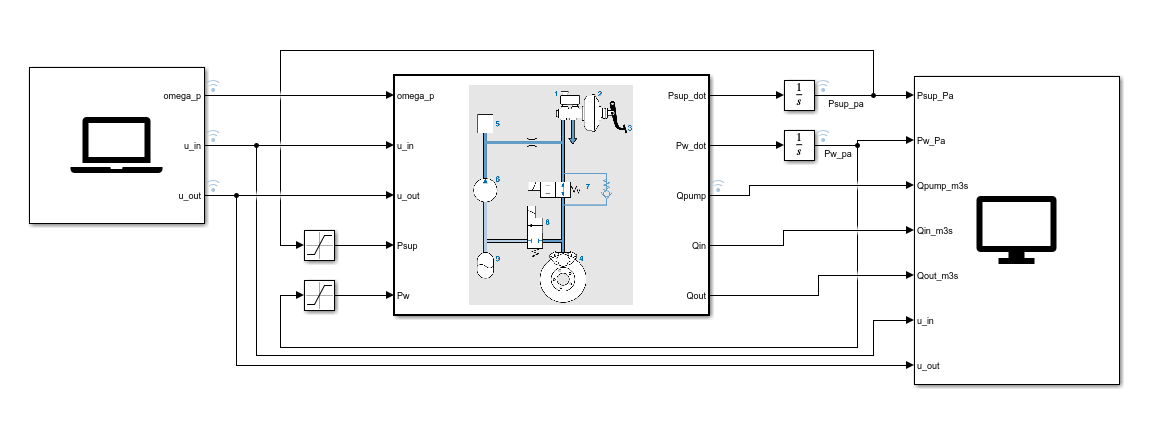
\includegraphics[width=0.8\textwidth]{figuras/image_matlab_function_bloco_hidraulico_2p.png}
    \fonte{O Autor.}
\end{figure}

As simulações são realizadas com integração numérica pelo solver \texttt{ode15s}, considerando como entradas as sequências temporais para a velocidade da bomba $\omega_p(t)$ e para as aberturas hidráulicas efetivas $u_{in}(t)$ e $u_{out}(t)$. As saídas analisadas incluem as pressões $P_{sup}(t)$ e $P_w(t)$, bem como as vazões internas $Q_{pump}(t)$, $Q_{in}(t)$ e $Q_{out}(t)$. Para facilitar a interpretação, as pressões são apresentadas como pressão \textit{gauge} em bar, conforme a relação
\begin{equation}
    P_{g}(t) = \frac{P(t)-P_{ret}}{10^5}\ \ [\text{bar}].
    \label{eq:pressao_gauge_bar}
\end{equation}

A metodologia adotada é análoga à utilizada em trabalhos experimentais com unidades hidráulicas de ESC/ABS, nos quais o comportamento de pressurização e alívio é avaliado a partir de perfis simples de comando em bomba e válvulas \cite{ZengYangHuang2023,Lv2014,HouhuaJing2022}. No presente trabalho, utiliza-se um ensaio integrado em malha aberta, combinando em uma única simulação três fases sequenciais: (i) pressurização, (ii) retenção e (iii) alívio.

O ensaio integrado é definido da seguinte forma:

\begin{itemize}
    \item \textbf{Fase A — pressurização}: a bomba é acionada com $\omega_p(t)$ assumindo valores em degrau, enquanto a válvula de entrada permanece totalmente aberta ($u_{in}=1$) e a válvula de saída permanece fechada ($u_{out}=0$). Nesta fase, espera-se que as pressões $P_{sup}$ e $P_w$ aumentem em patamares, com $P_w$ acompanhando o crescimento de $P_{sup}$ via transferência de fluido através da válvula de entrada.

    \item \textbf{Fase B — retenção}: a partir de um instante pré-definido, a bomba é desligada ($\omega_p=0$) e ambas as válvulas são fechadas ($u_{in}=0$, $u_{out}=0$). Nessa condição, o fluido permanece aprisionado no volume $V_w$, de modo que $P_w$ tende a manter-se próxima ao último patamar atingido, enquanto $P_{sup}$ decai gradualmente em direção a $P_{ret}$ devido ao vazamento interno no lado de suprimento.

    \item \textbf{Fase C — alívio}: por fim, mantém-se $\omega_p=0$ e $u_{in}=0$, abrindo-se a válvula de saída com $u_{out}>0$ em degrau. Espera-se uma queda monotônica de $P_w$ em direção a $P_{ret}$, com taxa de queda dependente da abertura efetiva da válvula de saída e compatível com a lei de orifício adotada para $Q_{out}$.
\end{itemize}

A Figura~\ref{fig:ensaio_malha_aberta_integrado} apresenta um resultado representativo do ensaio em malha aberta Codigo~\ref{cod:ensaio_integrado_malha_aberta}, mostrando as entradas ($\omega_p$, $u_{in}$, $u_{out}$), as pressões ($P_{sup}$ e $P_w$) e as vazões internas ($Q_{pump}$, $Q_{in}$ e $Q_{out}$).

\begin{figure}[htbp]
    \centering
    \caption{Ensaio integrado em malha aberta do subsistema hidráulico (entradas, pressões e vazões).}
    \label{fig:ensaio_malha_aberta_integrado}
    \IfFileExists{figuras/ensaio_malha_aberta_integrado.png}{%
        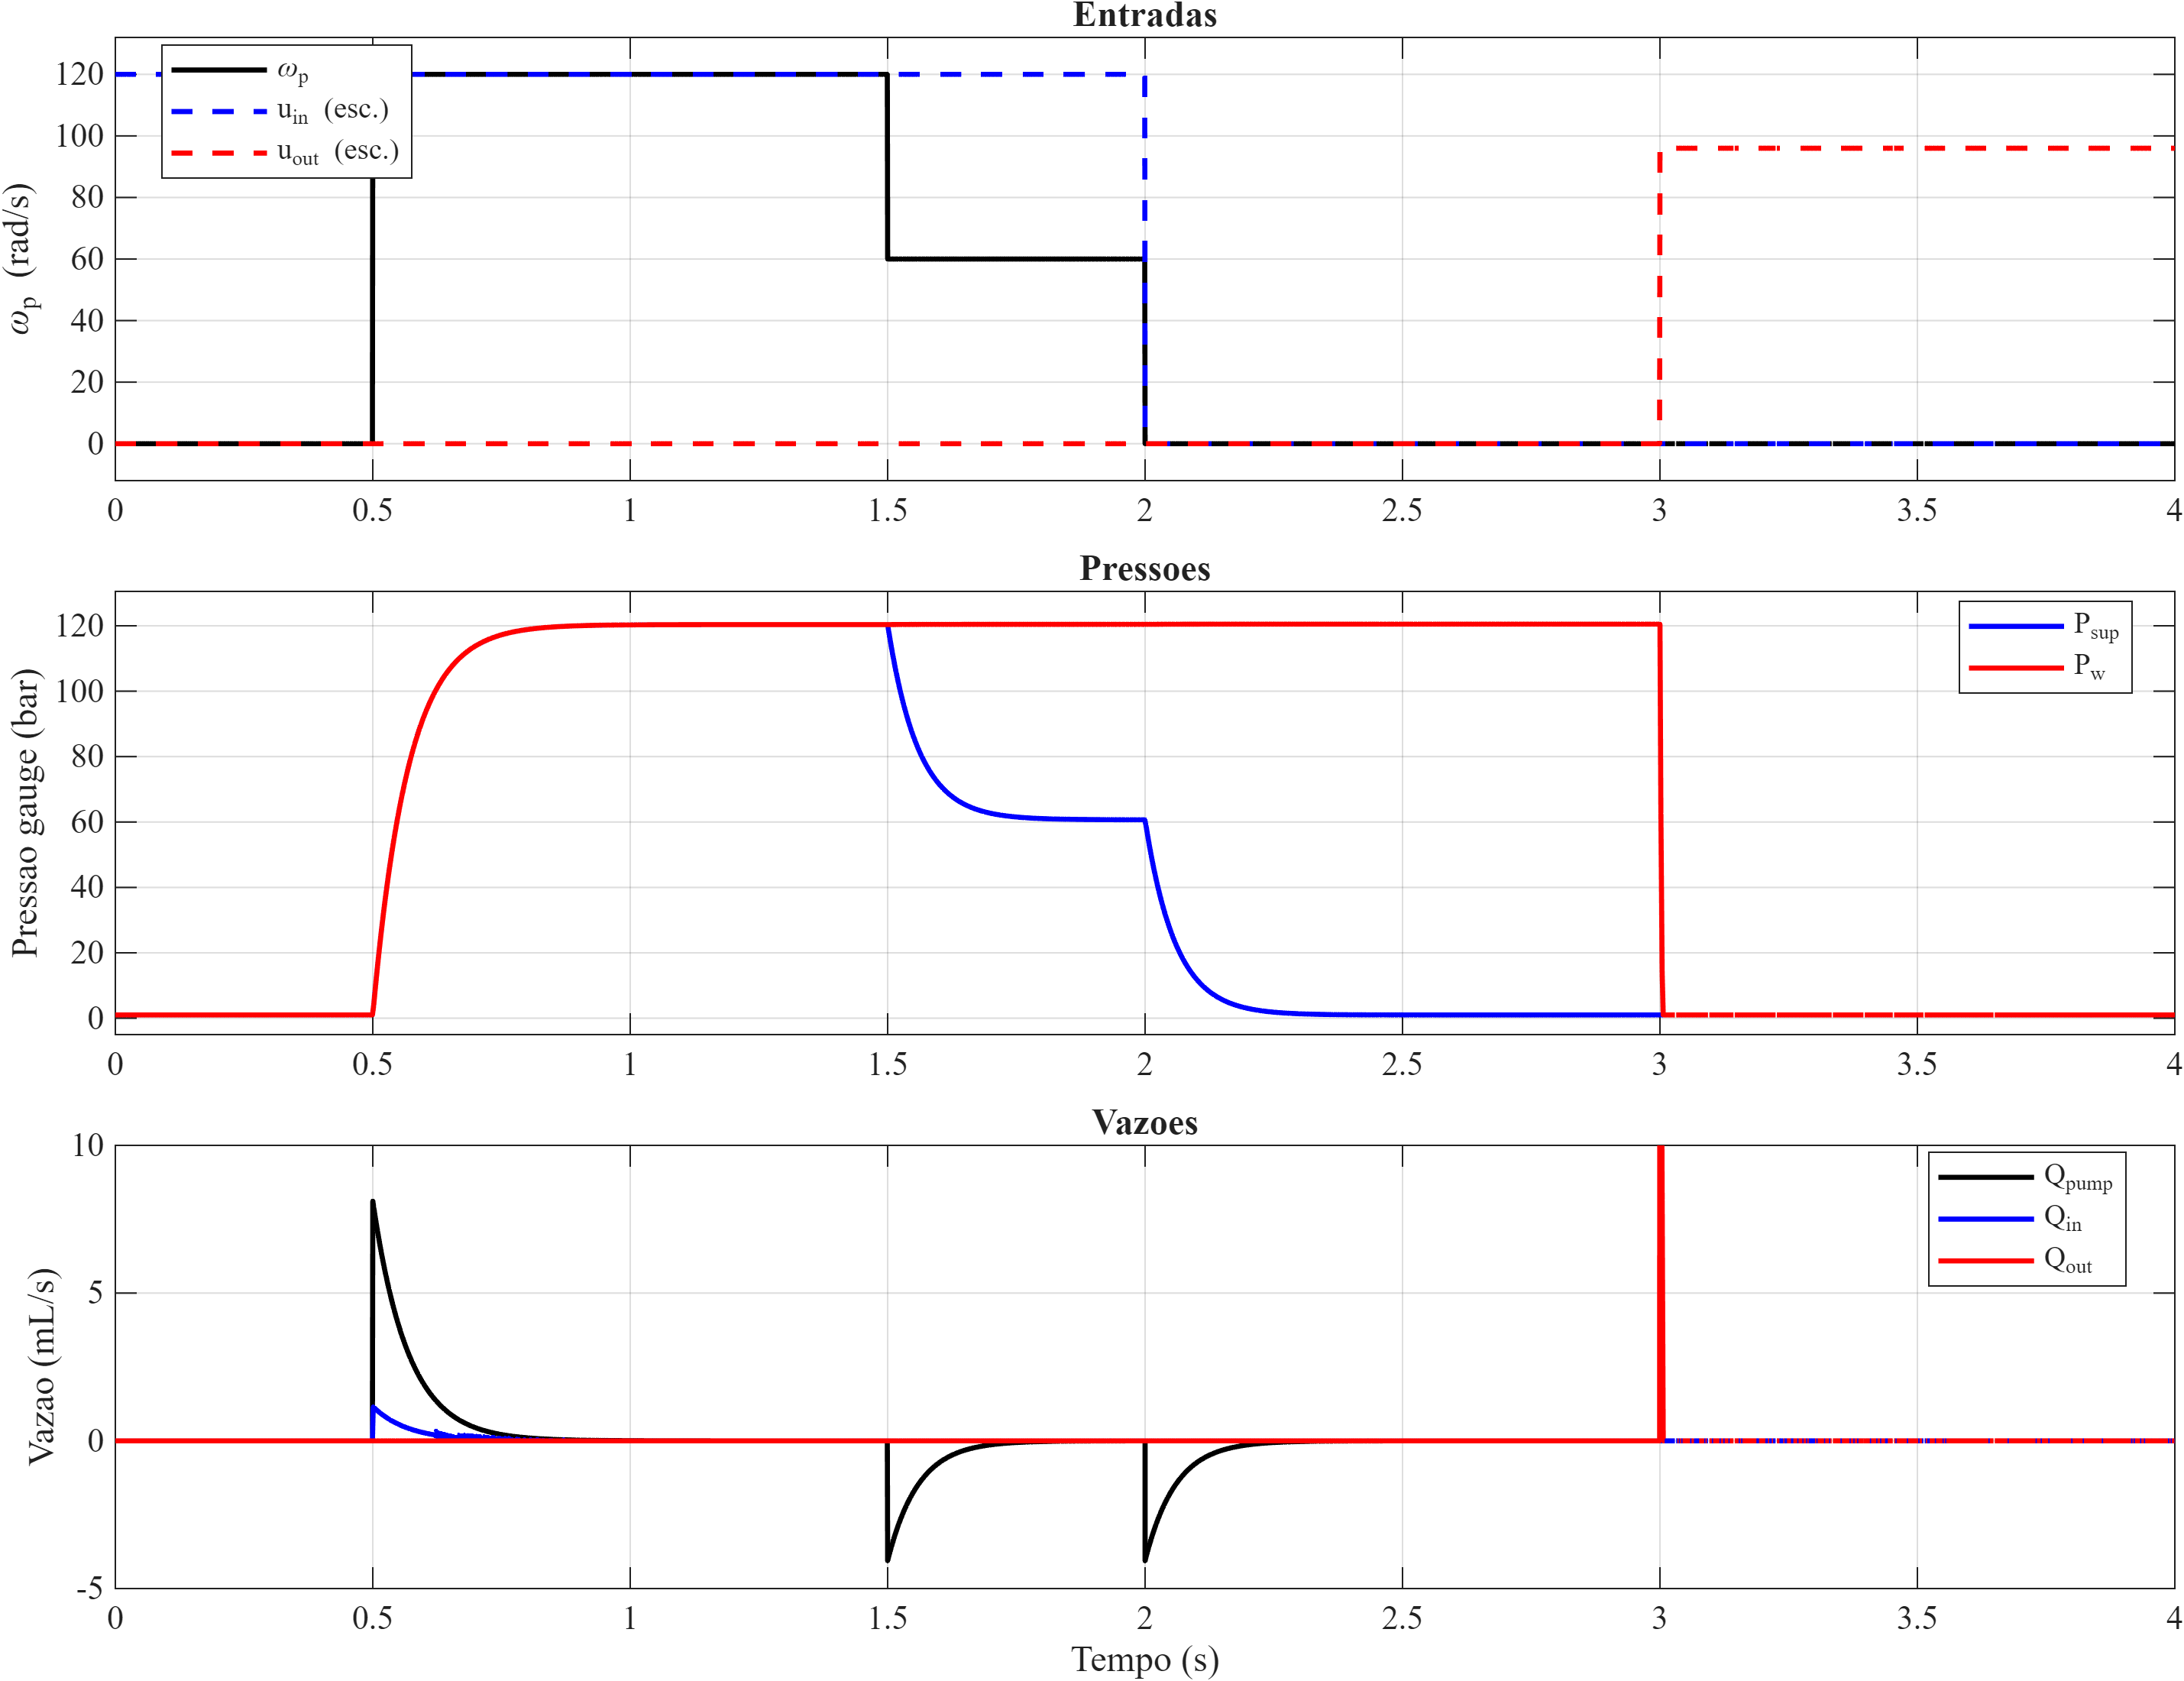
\includegraphics[width=0.9\textwidth]{figuras/ensaio_malha_aberta_integrado.png}%
    }{%
        \fbox{\parbox{0.9\textwidth}{\centering Figura a inserir: \texttt{figuras/ensaio\_malha\_aberta\_integrado.png}}}%
    }
    \fonte{O Autor.}
\end{figure}



%####################################################################
%####################################################################
%####################################################################
%####################################################################
\subsection{Ajuste de Parâmetros}
\label{sec:controle-ajuste-parametros-realistas}

Os resultados dos ensaios em malha aberta apresentados anteriormente indicam que o modelo hidráulico em duas pressões reproduz de forma qualitativa os comportamentos esperados de pressurização, retenção e alívio no circuito de roda. Entretanto, as amplitudes de pressão obtidas no caso base situam-se em torno de poucos bar, o que é adequado para a validação estrutural do modelo, mas abaixo das faixas tipicamente observadas em sistemas de freio automotivos reais.

Trabalhos experimentais com unidades hidráulicas de ESC/ABS reportam pressões no lado de suprimento da ordem de 8–13~MPa e variações rápidas de pressão no cilindro da roda, compatíveis com atuadores utilizados em frenagens ABS e ESC \cite{ZengYangHuang2023,DesignESCUnitTestSystem2018,HouhuaJing2022}. Em estudos de válvulas proporcionais e solenóides para atuadores de freio, são consideradas vazões máximas da ordem de 0,5–1{,}0~L/min para diferenças de pressão de dezenas de bar \cite{ProportionalPressureABS2023,ChenLv2017}, o que reforça a necessidade de calibrar o modelo concentrado para faixas de pressão mais elevadas.

Com o objetivo de aproximar o modelo das ordens de grandeza reportadas na literatura, este trabalho adota um segundo conjunto de parâmetros hidráulicos, mantida a estrutura do modelo em duas pressões, mas com volumes equivalentes e parâmetros de bomba ajustados. A Tabela~\ref{tab:parametros_hidraulico_realista} apresenta o conjunto de parâmetros utilizado nesta configuração ``realista'', a partir de adaptações das ordens de grandeza discutidas em \citeonline{ZengYangHuang2023,ProportionalPressureABS2023,Lv2014,ChenLv2017}.

\begin{table}[htbp]
\Caption{\label{tab:parametros_hidraulico_realista} Parâmetros ajustados para faixa de pressão realista}
\UNIFORtab{}{
    \begin{tabular}{ l | l | l | l }
        \hline Parâmetro & Símbolo & Valor adotado & Unidade \\
        \hline Densidade do fluido & $\rho$ & 850 & kg/m³ \\
        \hline Módulo volumétrico efetivo & $\beta$ & $1{,}5 \times 10^9$ & Pa \\
        \hline Pressão de retorno (referência) & $P_{ret}$ & $1{,}0 \times 10^5$ & Pa \\
        \hline Volume equivalente do suprimento & $V_{sup}$ & $5{,}0 \times 10^{-7}$ & m³ \\
        \hline Volume equivalente do canal/roda & $V_{w}$ & $5{,}0 \times 10^{-8}$ & m³ \\
        \hline Deslocamento volumétrico da bomba (por volta) & $D_p$ & $1{,}0 \times 10^{-5}$ & m³/rev \\
        \hline Eficiência volumétrica da bomba & $\eta_v$ & 0{,}85 & — \\
        \hline Coeficiente de descarga (orifício) & $C_d$ & 0{,}62 & — \\
        \hline Área efetiva máxima (válvula de entrada) & $A_{in,\max}$ & $1{,}0 \times 10^{-7}$ & m² \\
        \hline Área efetiva máxima (válvula de saída) & $A_{out,\max}$ & $1{,}0 \times 10^{-7}$ & m² \\
        \hline Coeficiente de vazamento interno (bomba) & $K_{lb}$ & $1{,}0 \times 10^{-11}$ & (m³/s)/Pa \\
        \hline
    \end{tabular}
}{\Fonte{Elaborado pelo autor, com base em \cite{ZengYangHuang2023,ProportionalPressureABS2023,Lv2014,ChenLv2017}.}}
\end{table}

Em comparação com o conjunto de parâmetros base, os volumes equivalentes $V_{sup}$ e $V_w$ foram reduzidos em aproximadamente duas ordens de grandeza, enquanto o deslocamento volumétrico da bomba $D_p$ foi aumentado. Essas alterações elevam a taxa de variação de pressão para uma faixa na ordem de dezenas de bar quando a bomba é acionada, mantendo as vazões instantâneas $Q_{pump}$, $Q_{in}$ e $Q_{out}$ dentro dos intervalos observados para válvulas e bombas de unidades hidráulicas automotivas \cite{ProportionalPressureABS2023,ChenLv2017,MotorParametricDesign2023}.

Para manter a clareza entre as duas configurações, o modelo ajustado foi implementado em uma segunda função MATLAB (\texttt{Bloco\_Hidraulico\_2P\_real}) e ensaiado com o mesmo perfil integrado em malha aberta descrito na Seção~\ref{sec:controle-ensaio-integrado}. As curvas resultantes apresentam pressões $P_w$ na faixa de aproximadamente 50–60~bar, em boa concordância com as ordens de grandeza reportadas em \citeonline{ZengYangHuang2023,DesignESCUnitTestSystem2018,HouhuaJing2022}. A Figura~\ref{fig:ensaio_malha_aberta_integrado_realista} ilustra os resultados obtidos com o modelo ajustado, evidenciando a capacidade de pressurização e alívio do sistema dentro de faixas realistas.

\begin{figure}[htbp]
    \centering
    \caption{Ensaio integrado em malha aberta do subsistema hidráulico (entradas, pressões e vazões) realista.}
    \label{fig:ensaio_malha_aberta_integrado_realista}
    \IfFileExists{figuras/ensaio_malha_aberta_integrado_real.png}{%
        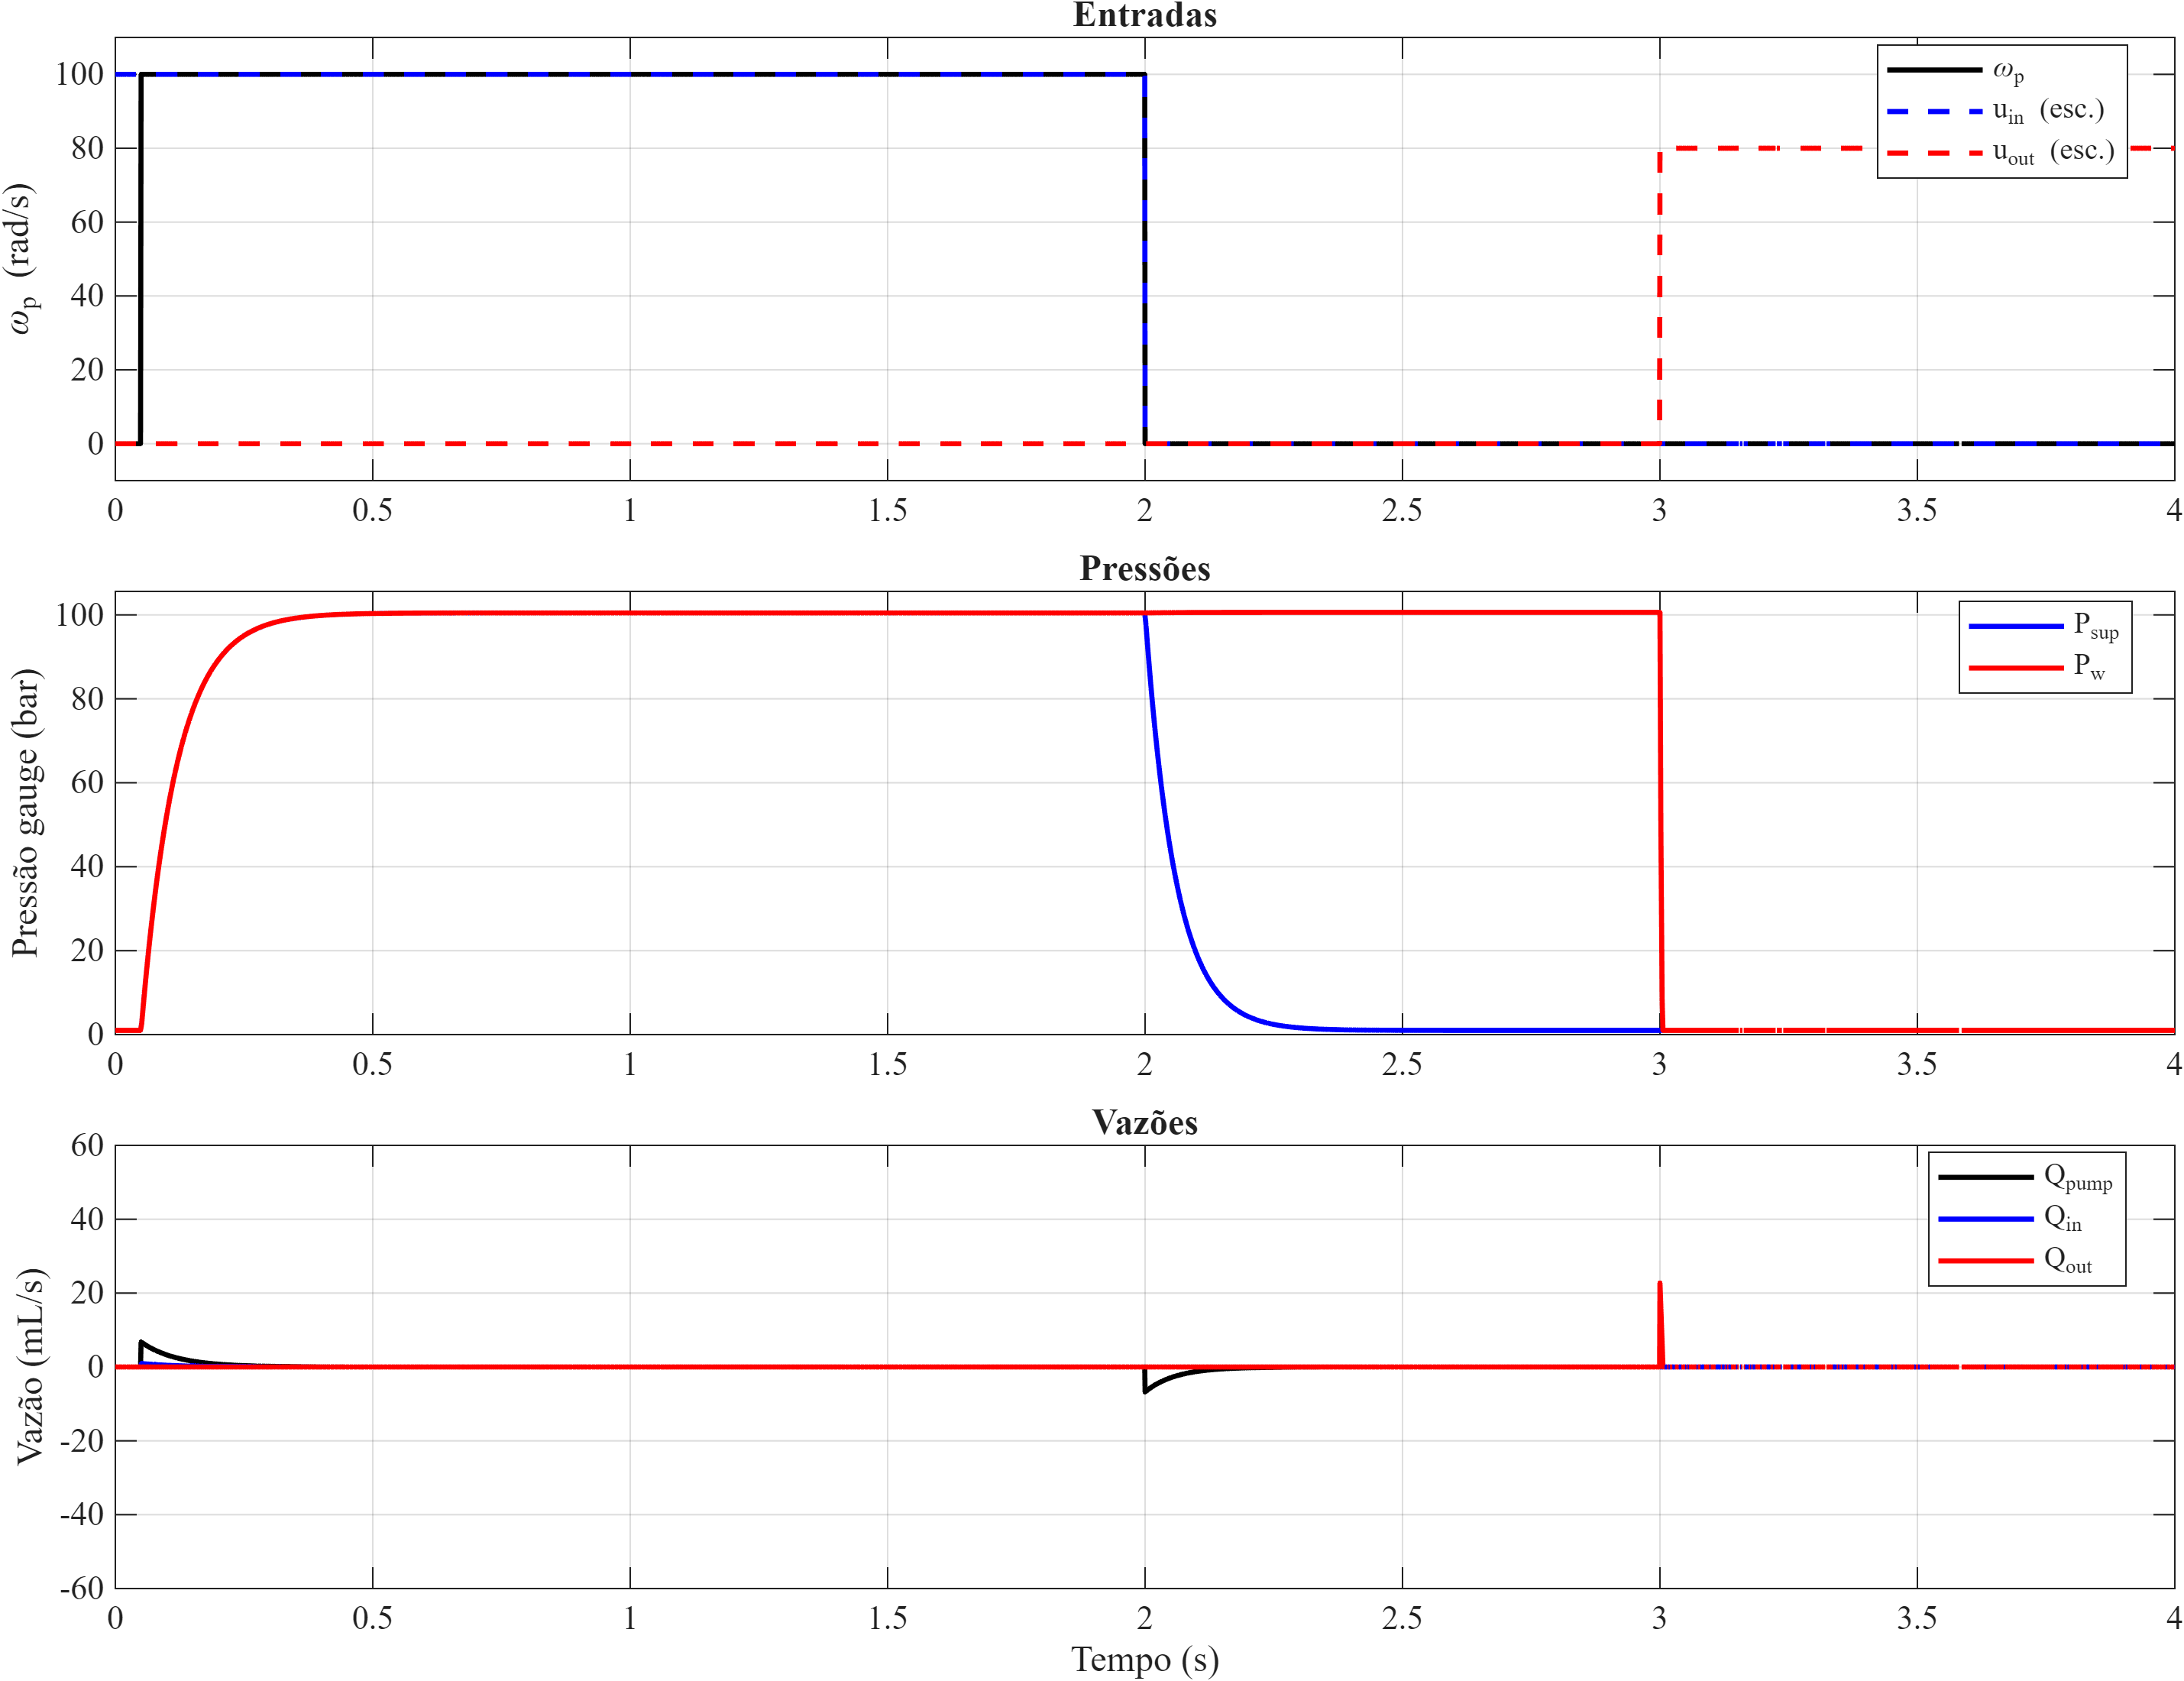
\includegraphics[width=0.9\textwidth]{figuras/ensaio_malha_aberta_integrado_real.png}%
    }{%
        \fbox{\parbox{0.9\textwidth}{\centering Figura a inserir: \texttt{figuras/ensaio\_malha\_aberta\_integrado\_real.png}}}%
    }
    \fonte{O Autor.}
\end{figure}

Além disso, as vazões máximas de bomba obtidas situam-se em torno de 60~mL/s, valores compatíveis com as capacidades de unidades hidráulicas estudadas em \citeonline{ProportionalPressureABS2023,ChenLv2017,MotorParametricDesign2023}.

Na continuidade deste capítulo, a síntese do controlador em espaço de estados poderá se apoiar em qualquer uma das duas configurações de parâmetros (caso base ou caso realista), dependendo do objetivo da simulação: análise didática da estrutura do modelo ou avaliação mais próxima das condições de operação de um sistema de freio automotivo real.


%####################################################################
%####################################################################
%####################################################################
%####################################################################
\subsection{Síntese da Validação do Modelo}
\label{sec:controle-sintese-validacao}

Os ensaios em malha aberta realizados com o modelo hidráulico em duas pressões permitem avaliar, em duas etapas complementares, a adequação da planta adotada para fins de projeto de controle de pressão.

Na primeira etapa, utilizando o conjunto de parâmetros base (Seção~\ref{sec:controle-4-1-5}), o objetivo principal foi verificar a coerência estrutural do modelo: causalidade entre entradas e saídas, saturações e sinais de vazão consistentes. O ensaio integrado em malha aberta (Seção~\ref{sec:controle-ensaio-integrado}) evidenciou:

\begin{itemize}
    \item um aumento de pressão no canal da roda $P_w$ durante a fase de pressurização, com $P_w$ acompanhando $P_{sup}$ enquanto a bomba é acionada e a válvula de entrada permanece aberta;

    \item a manutenção aproximada do patamar de pressão em $P_w$ na fase de retenção, quando o fluido permanece aprisionado no volume $V_w$ (bomba desligada e válvulas fechadas), em concordância com a ausência de caminho de descarga e de vazamentos significativos;

    \item uma queda controlada de $P_w$ em direção a $P_{ret}$ na fase de alívio, quando a válvula de saída é aberta, com taxa de queda compatível com a lei de orifício adotada para $Q_{out}$.
\end{itemize}

Embora, nessa configuração, as amplitudes de pressão permaneçam em uma faixa de poucos bar, o comportamento qualitativo observado é consistente com descrições experimentais de unidades hidráulicas ESC/ABS operando em regimes de pressurização e alívio \cite{ZengYangHuang2023,DesignESCUnitTestSystem2018,HouhuaJing2022,Lv2014}. Essa etapa confirma que a estrutura do modelo 2P é fisicamente coerente e adequada para representar o subsistema hidráulico de forma concentrada.

Na segunda etapa, foram ajustados os volumes equivalentes ($V_{sup}$ e $V_w$) e os parâmetros da bomba ($D_p$ e $K_{lb}$), conforme detalhado na Seção~\ref{sec:controle-ajuste-parametros-realistas}, de modo a aproximar as ordens de grandeza de pressão e vazão das reportadas na literatura para unidades hidráulicas automotivas reais \cite{ZengYangHuang2023,ProportionalPressureABS2023,ChenLv2017,MotorParametricDesign2023}. Com esse conjunto de parâmetros, o mesmo ensaio integrado em malha aberta produz pressões $P_w$ na faixa de aproximadamente 50–60~bar e vazões de bomba em torno de 60~mL/s, valores compatíveis com aqueles observados em testes experimentais de HCUs ESC/ABS \cite{ZengYangHuang2023,DesignESCUnitTestSystem2018,HouhuaJing2022}.

Dessa forma, o modelo hidráulico em duas pressões demonstra ser capaz de representar tanto o comportamento qualitativo quanto as ordens de grandeza relevantes do subsistema de freio, em consonância com trabalhos de referência na área. Essa validação em malha aberta, em conjunto com a calibração de parâmetros baseada na literatura, fornece uma base sólida para utilizar o modelo como planta no projeto de controladores em espaço de estados (LQR) e observadores de Luenberger, que serão tratados nas seções subsequentes.

%####################################################################
%####################################################################
%####################################################################
%####################################################################

\section{Linearização do Modelo Não Linear}
\label{sec:controle-linearizacao-2p}

%####################################################################
%####################################################################
%####################################################################
%####################################################################
\subsection{Definição do Ponto de Operação}
\label{sec:definicao-ponto-operacao}

Posteriormente, escolheu-se um ponto de operação $(x_0,u_0)$ representativo de uma situação de frenagem com pressão elevada (faixa de dezenas de bar em $P_{sup}$ e $P_w$, com $\omega_p$, $u_{in}$ e $u_{out}$ constantes e compatíveis com o ensaio realista em malha aberta). Os valores numéricos desse ponto e dos parâmetros físicos foram reunidos em uma estrutura de dados, e as jacobianas simbólicas $A_{\text{sym}}$ e $B_{\text{sym}}$ foram avaliadas em $(x_0,u_0)$ por meio do comando \texttt{subs}, seguido de conversão para forma numérica com \texttt{double}. Dessa forma, obtiveram-se as matrizes numéricas $A$ e $B$.

%####################################################################
%####################################################################
%####################################################################
%####################################################################
\subsection{Derivação das Matrizes Jacobianas}
\label{sec:derivacao-matrizes-jacobianas}

Conforme apresentado na Seção~\ref{sec:controle-modelo-hidraulico-2p}, o subsistema hidráulico de freio é descrito por um modelo em duas pressões com dinâmica dada por
\[
    \dot{P}_{sup} = \frac{\beta}{V_{sup}}\big(Q_{pump} - Q_{in}\big), 
    \qquad
    \dot{P}_{w}   = \frac{\beta}{V_{w}}\big(Q_{in} - Q_{out}\big),
\]
em que $Q_{pump}$, $Q_{in}$ e $Q_{out}$ são as vazões da bomba, da válvula de entrada e da válvula de saída, respectivamente. No caso realista considerado (Seção~\ref{sec:controle-ajuste-parametros-realistas}), essas vazões são modeladas por
\[
    Q_{pump} = K_b\,\omega_p - K_{lb}\big(P_{sup} - P_{ret}\big),
\]
\[
    Q_{in} = C_{v,in}\,A_{in,\max}\,u_{in}
             \sqrt{\frac{2\big(P_{sup} - P_{w}\big)}{\rho}},
    \qquad
    Q_{out} = C_{v,out}\,A_{out,\max}\,u_{out}
             \sqrt{\frac{2\big(P_{w} - P_{ret}\big)}{\rho}},
\]
assumindo-se que $P_{sup} > P_{w} > P_{ret}$ no ponto de operação considerado, de modo que os argumentos das funções raiz quadrada sejam positivos.

Para fins de projeto de controladores em espaço de estados, é conveniente dispor de uma aproximação linear do modelo em torno de um ponto de operação $(x_0,u_0)$. Define-se o vetor de estados como
\[
    x(t) = 
    \begin{bmatrix}
        P_{sup}(t) \\
        P_{w}(t)
    \end{bmatrix},
\]
e o vetor de entradas como
\[
    u(t) = 
    \begin{bmatrix}
        \omega_p(t) \\
        u_{in}(t) \\
        u_{out}(t)
    \end{bmatrix}.
\]
As equações não lineares podem ser escritas de forma compacta como
\[
    \dot{x}(t) = f\big(x(t),u(t)\big),
\]
em que $f(\cdot)$ agrega as expressões de $\dot{P}_{sup}$ e $\dot{P}_{w}$ em função de $x$ e $u$.

\subsubsection*{Derivadas parciais e forma linear aproximada}

A ideia central da linearização é aproximar a dinâmica não linear por um modelo linear em torno de um ponto de operação $(x_0,u_0)$, por meio das derivadas parciais de $f(x,u)$ com respeito aos estados e às entradas. Em termos gerais, deseja-se obter uma equação linear da forma
\[
    \frac{d\,\Delta x(t)}{dt} = A\,\Delta x(t) + B\,\Delta u(t),
\]
em que
\[
    \Delta x(t) = x(t) - x_0, \qquad
    \Delta u(t) = u(t) - u_0,
\]
e as matrizes $A$ e $B$ são dadas pelas derivadas parciais de $f$ avaliadas no ponto de operação:
\[
    A = \left.\frac{\partial f}{\partial x}\right|_{x_0,u_0},
    \qquad
    B = \left.\frac{\partial f}{\partial u}\right|_{x_0,u_0}.
\]
Essa forma é útil porque:
\begin{itemize}
    \item permite o uso direto de ferramentas de controle linear, como o Regulador Linear Quadrático (LQR);
    \item é válida em torno de um ponto de operação (equilíbrio ou condição estacionária);
    \item as variáveis $\Delta x$ e $\Delta u$ representam pequenas variações em torno dos valores de operação $x_0$ e $u_0$, o que é compatível com o conceito de controle em torno de um ponto de trabalho fixo.
\end{itemize}

Para ilustrar o procedimento, considere uma forma escalar simplificada da dinâmica da pressão,
\[
    \dot{P} = f\big(P, v_{out}, v_{in}\big)
             = \frac{\beta_e}{V}\left( K_b\,v_{in}
               - C_d A_{\max} v_{out}\sqrt{\frac{2P}{\rho}} \right),
\]
na qual $P$ representa a pressão na câmara hidráulica, $v_{in}$ é o sinal de comando da bomba e $v_{out}$ o sinal de comando de uma válvula proporcional de saída. Deseja-se obter um modelo linear aproximado da forma
\[
    \frac{d\,\Delta P}{dt}
    = A\,\Delta P + B_1\,\Delta v_{in} + B_2\,\Delta v_{out},
\]
em que $\Delta P = P - P_0$, $\Delta v_{in} = v_{in} - v_{in,0}$ e $\Delta v_{out} = v_{out} - v_{out,0}$ são as variações em torno do ponto de operação $(P_0, v_{out,0}, v_{in,0})$.

Aplicando derivadas parciais, obtêm-se os coeficientes da dinâmica linearizada:
\[
    A = \left.\frac{\partial f}{\partial P}\right|_{P_0,v_{out,0},v_{in,0}}
      = -\,\frac{\sqrt{2}\,A_{\max}\,C_d\,\beta_e\,v_{out,0}}{2\,V}
         \sqrt{\frac{1}{\rho P_0}},
\]
\[
    B_1 = \left.\frac{\partial f}{\partial v_{in}}\right|_{P_0,v_{out,0},v_{in,0}}
        = \frac{\beta_e\,K_b}{V},
\]
\[
    B_2 = \left.\frac{\partial f}{\partial v_{out}}\right|_{P_0,v_{out,0},v_{in,0}}
        = -\,\frac{\sqrt{2}\,A_{\max}\,C_d\,\beta_e}{V}
            \sqrt{\frac{P_0}{\rho}}.
\]
Substituindo essas derivadas na expressão linear, chega-se à forma
\[
    \frac{d\,\Delta P}{dt}
    = A\,\Delta P + B_1\,\Delta v_{in} + B_2\,\Delta v_{out},
\]
que é uma aproximação linear do comportamento da pressão em torno do ponto $(P_0, v_{out,0}, v_{in,0})$. Em princípio, esse desenvolvimento poderia ser repetido para todas as componentes de $f(x,u)$, de modo a obter explicitamente todas as entradas da matriz $A$ (derivadas em relação aos estados) e da matriz $B$ (derivadas em relação às entradas).

\subsubsection*{Uso do jacobiano simbólico no MATLAB}

No entanto, devido à presença de termos de raiz quadrada e de produtos entre variáveis e parâmetros, as expressões analíticas completas para todas as derivadas parciais tornam-se extensas e propensas a erro algébrico quando calculadas manualmente. Para evitar esse problema e manter o foco nas interpretações físicas e no projeto de controle, neste trabalho as derivadas parciais foram calculadas de forma simbólica no MATLAB, utilizando o operador jacobiano.

Inicialmente, foram definidas simbolicamente as variáveis de estado, de entrada e os parâmetros do modelo:
\[
    P_{sup},\, P_w,\, \omega_p,\, u_{in},\, u_{out},\,
    \beta,\, V_{sup},\, V_w,\, \rho,\, P_{ret},\,
    K_b,\, K_{lb},\, C_{v,in},\, A_{in,\max},\, C_{v,out},\, A_{out,\max}.
\]
Em seguida, construíram-se simbolicamente as expressões de $Q_{pump}$, $Q_{in}$, $Q_{out}$ e dos termos $\dot{P}_{sup}$ e $\dot{P}_{w}$, agrupando-os no vetor
\[
    f(x,u) =
    \begin{bmatrix}
        \dot{P}_{sup} \\
        \dot{P}_{w}
    \end{bmatrix}.
\]
A partir dessa definição, as matrizes de derivadas parciais simbólicas (jacobianas) em relação aos estados e às entradas foram determinadas por
\[
    A_{\text{sym}} = \frac{\partial f}{\partial x},
    \qquad
    B_{\text{sym}} = \frac{\partial f}{\partial u},
\]
utilizando o comando \texttt{jacobian} do MATLAB.

A matriz de saída foi definida como
\[
    C = \begin{bmatrix} 0 & 1 \end{bmatrix},
\]
uma vez que a saída de interesse é a pressão no canal da roda $P_w$, e admitiu-se que a saída não depende diretamente das entradas no ponto de operação, de modo que
\[
    D = \begin{bmatrix} 0 & 0 & 0 \end{bmatrix}.
\]

O sistema linearizado em espaço de estados foi então construído no MATLAB por meio do comando
\[
    \texttt{sys\_lin = ss(A,B,C,D)},
\]
resultando no seguinte conjunto de matrizes:
\[
    A =
    10^{5}
    \begin{bmatrix}
        -0{,}3000 + 0{,}1427\,\mathrm{i} & \phantom{-}0{,}0000 - 0{,}1427\,\mathrm{i} \\
        \phantom{-}0{,}0000 - 1{,}4266\,\mathrm{i} & \phantom{-}0{,}0000 + 1{,}4266\,\mathrm{i}
    \end{bmatrix},
\]
\[
    B =
    10^{11}
    \begin{bmatrix}
        \phantom{-}0{,}0406 & \phantom{-}0{,}0000 - 0{,}0285\,\mathrm{i} & \phantom{-}0{,}0000 \\
        \phantom{-}0{,}0000 & \phantom{-}0{,}0000 + 0{,}2853\,\mathrm{i} & -2{,}1159
    \end{bmatrix},
\]
\[
    C = \begin{bmatrix} 0 & 1 \end{bmatrix},
    \qquad
    D = \begin{bmatrix} 0 & 0 & 0 \end{bmatrix}.
\]
As pequenas partes imaginárias presentes em alguns elementos de $A$ e $B$ são resultado de arredondamentos numéricos do cálculo simbólico e podem ser desprezadas na interpretação física, sendo o sistema efetivamente real.

Os polos do modelo linearizado são obtidos a partir dos autovalores de $A$:
\[
    p_1 \approx -2{,}73\times 10^{4},
    \qquad
    p_2 \approx -2{,}65\times 10^{3},
\]
ambos localizados no semiplano esquerdo do plano-$s$, o que indica que o sistema linearizado é localmente estável em torno do ponto de operação considerado. O polo mais rápido ($p_1$) está associado a uma dinâmica de alta frequência (resposta mais rígida da pressão no suprimento), enquanto o polo mais lento ($p_2$) está relacionado à dinâmica da pressão no canal da roda, ainda rápida em termos absolutos, mas menos rígida que a do suprimento. Essa separação de escalas de tempo é coerente com as simulações apresentadas na Seção~\ref{sec:controle-ajuste-parametros-realistas}, nas quais observa-se uma rápida convergência da pressão para o patamar desejado, sem oscilações excessivas.

\subsubsection*{Análise dos polos e resposta em frequência}

A partir do sistema linearizado $\texttt{sys\_lin}$, foi construído o diagrama de polos no plano-$s$ (Figura~\ref{fig:mapa_de_carno}), utilizando o comando \texttt{pzmap} do MATLAB. Nessa figura, observam-se dois polos reais localizados no semiplano esquerdo, com módulos da ordem de $10^{3}$ e $10^{4}$~rad/s. A ausência de polos no semiplano direito confirma a estabilidade local do modelo linearizado. Além disso, a diferença entre os módulos dos polos evidencia a existência de uma dinâmica dominante mais lenta (associada à variação de $P_w$) e de uma dinâmica mais rápida (associada ao acoplamento com $P_{sup}$), o que justifica a escolha de horizontes de tempo e de frequências de amostragem compatíveis com a banda de atuação do controlador de pressão.

Complementarmente, foi analisada a resposta em frequência entre as entradas hidráulicas de interesse e a pressão no canal da roda $P_w$. A Figura~\ref{fig:diagrama_de_bode} apresenta o diagrama de Bode da função de transferência entre a abertura da válvula de entrada $u_{in}$ e a pressão $P_w$, obtida a partir do subsistema SISO correspondente de $\texttt{sys\_lin}$. Observa-se que:
\begin{itemize}
    \item o ganho em baixa frequência é elevado, indicando que variações quase estacionárias em $u_{in}$ resultam em variações significativas da pressão $P_w$;
    \item a frequência de corte situa-se em uma faixa compatível com a dinâmica desejada para o controle de frenagem, permitindo que o sistema acompanhe comandos de pressão dentro da banda de interesse do controlador;
    \item a fase apresenta um comportamento típico de sistema de segunda ordem, sem inversões bruscas, o que contribui para a robustez do projeto de controle em malha fechada.
\end{itemize}

Assim, a linearização do modelo hidráulico em duas pressões por meio das derivadas parciais (implementadas simbolicamente via jacobiano no MATLAB) resultou em um sistema linear localmente estável, com polos e características de resposta em frequência coerentes com o comportamento observado nas simulações não lineares. Essa representação linearizada constitui a base para o projeto do regulador linear quadrático (LQR) e do observador de Luenberger apresentados nas seções subsequentes.


%####################################################################
%####################################################################
%####################################################################
%####################################################################
\subsection{Formulação em Espaço de Estados}
\label{sec:controle-formulacao-espaço-estados}
A partir do modelo linearizado descrito na Seção~\ref{sec:controle-linearizacao-2p}, o subsistema hidráulico pode ser representado em espaço de estados pela forma
\[
    \dot{x}(t) = A\,x(t) + B\,u(t), \qquad
    y(t) = C\,x(t),
\]
em que
\[
    x(t) = 
    \begin{bmatrix}
        P_{sup}(t) \\
        P_{w}(t)
    \end{bmatrix},
    \quad
    u(t) =
    \begin{bmatrix}
        \omega_p(t) \\
        u_{in}(t) \\
        u_{out}(t)
    \end{bmatrix},
    \quad
    y(t) = P_w(t).
\]

No contexto do controle de pressão nas rodas, a variável de interesse é a pressão no canal da roda $P_w$, que deve acompanhar uma referência de pressão $P_{w,\text{ref}}(t)$ gerada a partir da demanda de desaceleração do veículo (por exemplo, pelo controlador de ACC, conforme discutido na Seção~\ref{sec:controle-acc}). As entradas $u_{in}$ e $u_{out}$ representam respectivamente os comandos das válvulas de entrada e de saída do circuito hidráulico, enquanto $\omega_p$ está associada à velocidade de rotação da bomba.

Considerando que, na prática, a bomba tende a operar em uma faixa de rotação relativamente constante durante uma frenagem de serviço, adota-se neste trabalho que $\omega_p$ é mantida em torno de um valor nominal $\omega_{p,0}$, de forma que as principais ações de controle sobre a pressão $P_w$ são realizadas por meio de $u_{in}$ e $u_{out}$. Nesse caso, é conveniente reescrever o modelo em termos do vetor de entradas reduzido
\[
    u_c(t) =
    \begin{bmatrix}
        u_{in}(t) \\
        u_{out}(t)
    \end{bmatrix},
\]
e da matriz de entrada correspondente $B_c$, obtida a partir de $B$ pela seleção das colunas associadas a $u_{in}$ e $u_{out}$. A dinâmica em espaço de estados utilizada para o projeto de controle torna-se, então,
\[
    \dot{x}(t) = A\,x(t) + B_c\,u_c(t), \qquad
    y(t) = C\,x(t),
\]
com $x \in \mathbb{R}^2$, $u_c \in \mathbb{R}^2$ e $y \in \mathbb{R}$.

O objetivo de controle pode ser formulado como o rastreamento da pressão $P_w$ em torno de uma referência $P_{w,\text{ref}}$, garantindo:
\begin{itemize}
    \item erro de regime pequeno entre $P_w$ e $P_{w,\text{ref}}$;
    \item dinâmica de resposta adequada (tempo de subida e de acomodação compatíveis com as exigências de frenagem);
    \item esforço de controle moderado nas válvulas $u_{in}$ e $u_{out}$, evitando comutações excessivas e saturações.
\end{itemize}
Para atender a esses requisitos, será empregado um regulador linear quadrático (LQR) em espaço de estados, associado a um observador de Luenberger para estimação dos estados, conforme descrito na seção subsequente.

%####################################################################
%####################################################################
%####################################################################
%####################################################################
\subsection{Discussão Estrutural das Não Linearidades}

A dinâmica do sistema hidráulico é governada por relações constitutivas não lineares decorrentes do escoamento através de orifícios. Em particular, a vazão é modelada por

\begin{equation}
Q = C_v A \sqrt{\frac{2\Delta P}{\rho}},
\end{equation}

o que implica dependência não linear do tipo $\sqrt{\Delta P}$ entre as variáveis de estado.

Do ponto de vista estrutural, o sistema apresenta não linearidade de classe $C^1$, porém não afim nos estados. A matriz jacobiana do sistema depende explicitamente do ponto de operação por meio do termo

\begin{equation}
\frac{\partial Q}{\partial \Delta P} =
\frac{C_v A}{\rho}
\frac{1}{\sqrt{2\Delta P/\rho}},
\end{equation}

indicando que o ganho incremental do sistema varia inversamente com $\sqrt{\Delta P}$.

Consequentemente, o sistema não é globalmente linearizável por transformação de estados simples, e sua dinâmica efetiva depende fortemente do regime operacional. Tal característica impõe que qualquer projeto baseado em modelo linear represente apenas uma aproximação local do comportamento não linear.

%####################################################################
%####################################################################
%####################################################################
%####################################################################
\subsection{Região de Validade da Linearização}

A linearização foi realizada a partir da expansão em série de Taylor de primeira ordem do campo vetorial não linear

\begin{equation}
\dot{x} = f(x,u)
\end{equation}

em torno do ponto de equilíbrio $(x_0,u_0)$, resultando em

\begin{equation}
\dot{\tilde{x}} = A \tilde{x} + B \tilde{u},
\end{equation}

onde $\tilde{x} = x - x_0$ e $\tilde{u} = u - u_0$.

O erro de aproximação associado à truncagem da série é da ordem

\begin{equation}
\mathcal{O}(\|\tilde{x}\|^2),
\end{equation}

indicando que a validade do modelo linear depende diretamente da magnitude das perturbações.

Nas simulações realizadas, as variações de referência atingem amplitudes comparáveis ao próprio ponto de operação, o que implica que a hipótese de pequenas perturbações não é rigorosamente satisfeita. Ainda assim, observou-se estabilidade prática do sistema em malha fechada, o que sugere que a dinâmica dominante permanece capturada pela linearização dentro da faixa considerada.


%####################################################################
%####################################################################
%####################################################################
%####################################################################
\section{Projeto do Controlador LQR}
\label{sec:controle-lqr-luenberger}

\subsection{Definição das Matrizes de Peso}
\label{sec:definicao-matrizes-peso}

Com a representação em espaço de estados
\[
    \dot{x}(t) = A\,x(t) + B_c\,u_c(t), \qquad
    y(t) = C\,x(t),
\]
o controlador em espaço de estados adotado neste trabalho baseia-se em um regulador linear quadrático (LQR), complementado por um observador de Luenberger para estimação de estados não diretamente mensuráveis.

O regulador LQR tem como objetivo determinar uma lei de controle por realimentação de estados da forma
\[
    u_c(t) = -K\,\big(x(t) - x_{\text{ref}}\big),
\]
em que $K$ é a matriz de ganhos a ser projetada e $x_{\text{ref}}$ representa o estado de referência associado à pressão desejada na roda. No caso mais simples, pode-se considerar $x_{\text{ref}}$ como o vetor de estados correspondente a $P_{w,\text{ref}}$ no ponto de operação, de forma que o controlador atue para minimizar as variações em torno desse ponto.

O ganho $K$ é obtido pela minimização de uma função de custo quadrática do tipo
\[
    J = \int_{0}^{\infty}
        \Big[
            x(t)^{T} Q\,x(t)
            + u_c(t)^{T} R\,u_c(t)
        \Big]\,dt,
\]
em que $Q \succeq 0$ é a matriz de ponderação dos estados e $R \succ 0$ é a matriz de ponderação do esforço de controle. Intuitivamente, $Q$ penaliza desvios da pressão em relação ao valor desejado, enquanto $R$ penaliza variações e amplitudes excessivas nos comandos das válvulas $u_{in}$ e $u_{out}$. A escolha adequada de $Q$ e $R$ permite ajustar o compromisso entre desempenho (rapidez e precisão) e esforço de controle (limitação da atuação das válvulas).

\subsection{Cálculo do Ganho Ótimo}
\label{sec:calculo-ganho-otimo}

A solução ótima do problema LQR é dada por
\[
    K = R^{-1} B_c^{T} P,
\]
em que $P$ é a solução simétrica definida positiva da equação algébrica de Riccati
\[
    A^{T} P + P A - P B_c R^{-1} B_c^{T} P + Q = 0.
\]
No MATLAB, esse ganho é calculado diretamente por meio do comando \texttt{lqr(A,B\_c,Q,R)}, a partir das matrizes $A$, $B_c$, $Q$ e $R$ definidas para o modelo linearizado.

%####################################################################
%####################################################################
%####################################################################
%####################################################################
\section{Projeto do Observador de Luenberger}
\label{sec:projeto-observador-luenberger}

%####################################################################
%####################################################################
%####################################################################
%####################################################################
\subsection{Posicionamento de Polos}
\label{sec:posicionamento-polos}

Na prática, nem todos os estados do sistema são diretamente mensuráveis com boa qualidade. Em particular, a pressão no canal da roda $P_w$ é tipicamente disponível via sensor, enquanto a pressão no suprimento $P_{sup}$ pode não estar disponível ou estar sujeita a ruídos significativos. Para reconstruir o vetor de estados $x(t)$ a partir da medida de saída $y(t)$, emprega-se um observador de Luenberger.

A dinâmica do observador é dada por
\[
    \dot{\hat{x}}(t) = A\,\hat{x}(t) + B_c\,u_c(t)
                       + L\big(y(t) - \hat{y}(t)\big),
\]
\[
    \hat{y}(t) = C\,\hat{x}(t),
\]
em que $\hat{x}(t)$ é o vetor de estados estimados, $\hat{y}(t)$ é a saída estimada e $L$ é a matriz de ganhos do observador. O termo de correção $L\big(y - \hat{y}\big)$ atua de forma a forçar a convergência de $\hat{x}(t)$ para $x(t)$, compensando incertezas no modelo e efeitos de ruído de medição.

%####################################################################
%####################################################################
%####################################################################
%####################################################################
\subsection{Dinâmica do Erro de Estimação}
\label{sec:dinamica-erro-estimacao}

Definindo o erro de estimação como $e(t) = x(t) - \hat{x}(t)$, a dinâmica do erro é dada por
\[
    \dot{e}(t) = \big(A - L C\big)\,e(t).
\]
Assim, a estabilidade e a velocidade de convergência do observador dependem diretamente da escolha de $L$, que deve ser realizada de modo a posicionar os autovalores de $A - LC$ suficientemente à esquerda no plano-$s$. Na prática, escolhem-se polos do observador mais rápidos do que os polos da planta em malha fechada com o controlador LQR, de forma a garantir que a estimação dos estados seja bem mais rápida do que a atuação do controlador.

A matriz $L$ pode ser obtida por técnicas de alocação de polos, por exemplo, utilizando o comando \texttt{place} do MATLAB aplicado à transposta do par observável $(A^{T}, C^{T})$:
\[
    L^{T} = \texttt{place}\big(A^{T}, C^{T}, p_{\text{obs}}\big),
\]
em que $p_{\text{obs}}$ é o conjunto de polos desejados para o observador. Uma vez determinado $L$, a lei de controle implementada passa a ser
\[
    u_c(t) = -K\,\big(\hat{x}(t) - x_{\text{ref}}\big),
\]
utilizando os estados estimados $\hat{x}(t)$ no lugar dos estados reais $x(t)$, o que torna o controlador viável em uma implementação embarcada com sensores limitados.

A combinação do regulador LQR com o observador de Luenberger resulta, portanto, em um esquema de controle em espaço de estados que oferece:
\begin{itemize}
    \item desempenho ótimo em termos de compromisso entre erro de seguimento de pressão e esforço de controle;
    \item robustez a ruídos de medição e incertezas moderadas no modelo;
    \item viabilidade de implementação em microcontroladores automotivos, uma vez que as leis de controle e estimação são lineares e de baixa ordem.
\end{itemize}
Nas seções seguintes, são apresentados o ajuste dos parâmetros $Q$ e $R$, a escolha dos polos do observador e os resultados de simulação em malha fechada para o sistema hidráulico de freio.

%####################################################################
%####################################################################
%####################################################################
%####################################################################
\section{Discretização do Sistema}
\label{sec:discretizacao-sistema}

%####################################################################
%####################################################################
%####################################################################
%####################################################################
\subsection{Modelo Discreto}
\label{sec:modelo-discreto}

Para viabilizar a implementação do controlador em ambiente digital e sua integração ao modelo em Simulink com solver de passo fixo, o modelo em espaço de estados contínuo obtido a partir da linearização (Seção~\ref{sec:controle-linearizacao-2p}) foi discretizado com período de amostragem $T_s$.

Neste trabalho, adotou-se um período de amostragem da ordem de $T_s = 10^{-4}\,\text{s}$ (0{,}1~ms), compatível com a dinâmica rápida do subsistema hidráulico e com a necessidade de representar adequadamente os transitórios de pressão. A discretização foi realizada por retenção de ordem zero (\textit{zero-order hold}), conforme implementado no MATLAB pelo comando \texttt{c2d} aplicado ao sistema contínuo $\texttt{sys\_c}$.

O modelo discreto assume a forma
\begin{equation}
x(k+1) = A_d\,x(k) + B_d\,u(k),
\qquad
y(k) = C_d\,x(k),
\end{equation}
em que $x(k)$ representa o vetor de estados amostrado, $u(k)$ é a entrada discretizada e $y(k)$ é a saída de interesse (pressão no canal da roda). As matrizes $A_d$, $B_d$ e $C_d$ são obtidas diretamente do sistema discreto \texttt{sys\_d}.

%####################################################################
%####################################################################
%####################################################################
%####################################################################
\subsection{Projeto do LQR Discreto}
\label{sec:projeto-lqr-discreto}

Uma vez obtido o modelo discreto, o controlador LQR pode ser projetado diretamente no domínio discreto por meio da minimização de um funcional quadrático do tipo
\begin{equation}
J = \sum_{k=0}^{\infty} \left( x(k)^\top Q\,x(k) + u(k)^\top R\,u(k) \right),
\end{equation}
em que $Q \succeq 0$ e $R \succ 0$ definem o compromisso entre desempenho e esforço de controle.

O ganho discreto é obtido no MATLAB pelo comando \texttt{dlqr(\,A\_d,B\_d,Q,R\,)}, resultando em uma lei de controle do tipo
\begin{equation}
u(k) = -K_d\,x(k).
\end{equation}
Em aplicações de seguimento de referência, pode-se ainda empregar um pré-filtro (por exemplo, $N_r$) para ajuste do ganho estático em regime permanente. No escopo deste trabalho, o controle discreto utilizado nas simulações em malha fechada é estendido com ação integral (LQI), de modo a garantir eliminação do erro estacionário para referências constantes.

%####################################################################
%####################################################################
%####################################################################
%####################################################################
\subsection{Projeto do Observador Discreto}
\label{sec:projeto-observador-discreto}

Para estimar os estados do modelo discreto a partir da medida de saída $y(k)$, utiliza-se um observador de Luenberger no domínio discreto. A atualização do observador pode ser escrita como
\begin{equation}
\hat{x}(k+1) = A_d\,\hat{x}(k) + B_d\,u(k) + L_d\,\big(y(k) - \hat{y}(k)\big),
\qquad
\hat{y}(k) = C_d\,\hat{x}(k).
\end{equation}

Definindo o erro de estimação $e(k) = x(k) - \hat{x}(k)$, obtém-se a dinâmica
\begin{equation}
e(k+1) = \big(A_d - L_d C_d\big)\,e(k).
\end{equation}
Assim, a escolha de $L_d$ determina a velocidade de convergência do observador. Na implementação utilizada, $L_d$ é obtida por alocação de polos com o comando \texttt{place}, posicionando os polos do observador discretizado como uma fração dos polos de $A_d$, de forma a torná-los mais rápidos do que a dinâmica dominante do sistema.


%####################################################################
%####################################################################
%####################################################################
%####################################################################

\section{Projeto do Controlador LQI Discreto}
\label{sec:controle-lqi-discreto}

Após a síntese do controlador LQI discreto, procedeu-se à sua implementação na planta hidráulica não linear originalmente modelada. Diferentemente da etapa de projeto, baseada no modelo linearizado em torno do ponto de operação nominal, a validação foi realizada considerando integralmente as não linearidades do sistema, incluindo as relações quadráticas de vazão, os efeitos de compressibilidade do fluido e as restrições físicas impostas às pressões e atuadores.

%####################################################################
%####################################################################
%####################################################################
%####################################################################
\subsection{Sistema Aumentado com Ação Integral}

O sistema aumentado utilizado para a síntese do LQI é descrito por:

\begin{equation}
x_{aug}(k+1) =
\begin{bmatrix}
A_d & 0 \\
- C_d T_s & 1
\end{bmatrix}
x_{aug}(k)
+
\begin{bmatrix}
B_d \\
0
\end{bmatrix}
u(k)
\end{equation}

onde o estado adicional corresponde à integral do erro de rastreamento, definida por:

\begin{equation}
z(k+1) = z(k) + T_s \left( r(k) - y(k) \right)
\end{equation}

\subsubsection{Inclusão da Ação Integral}

Considere o sistema discreto

\begin{equation}
x(k+1) = A_d x(k) + B_d u(k),
\qquad
y(k) = C_d x(k).
\end{equation}

Define-se o estado integrador

\begin{equation}
z(k+1) = z(k) + T_s (r(k) - y(k)),
\end{equation}

resultando no sistema aumentado

\begin{equation}
x_{aug}(k+1) =
\begin{bmatrix}
A_d & 0 \\
- C_d T_s & 1
\end{bmatrix}
x_{aug}(k)
+
\begin{bmatrix}
B_d \\
0
\end{bmatrix}
u(k)
+
\begin{bmatrix}
0 \\
T_s
\end{bmatrix}
r(k).
\end{equation}

A inclusão do integrador introduz um polo unitário no sistema aumentado. A controlabilidade do par associado às matrizes do sistema aumentado foi verificada numericamente, garantindo viabilidade da síntese LQI.

Sob estabilidade da malha fechada, o teorema do valor final para sistemas discretos assegura que

\begin{equation}
\lim_{k \to \infty} e(k) = 0,
\end{equation}

desde que a referência seja constante e admissível.

A lei de controle implementada assume a forma:

\begin{equation}
u(k) = -K_x x(k) - K_i z(k)
\end{equation}

em que $K_x$ e $K_i$ foram obtidos por meio da solução da equação algébrica de Riccati discreta associada ao problema LQI.

\subsection{Cálculo dos Ganhos Kx e Ki}

A seleção das matrizes de ponderação do regulador LQI foi realizada considerando critérios físicos e numéricos. A matriz

\begin{equation}
Q_a = \mathrm{diag}(10^{-12}, 10^{-10}, 10^{4})
\end{equation}

atribui peso significativamente maior ao estado integrador, priorizando a eliminação do erro estacionário.

Os estados associados às pressões receberam ponderações menores devido às suas magnitudes físicas elevadas (ordem de $10^7$ Pa), evitando escalonamento inadequado no problema de otimização.

O parâmetro $R = 10^{-6}$ foi escolhido de modo a permitir ação de controle suficientemente energética sem penalizar excessivamente a rotação da bomba hidráulica. Valores menores de $R$ resultaram em maior esforço de controle e risco de saturação, enquanto valores maiores degradaram o desempenho de seguimento.

\subsubsection{Escolha das Matrizes de Ponderação}

O controlador LQI foi obtido pela minimização do funcional quadrático discreto

\begin{equation}
J = \sum_{k=0}^{\infty}
\left(
x_{aug}(k)^\top Q_a x_{aug}(k) +
u(k)^\top R u(k)
\right).
\end{equation}

A escolha de $R$ regula diretamente o compromisso entre desempenho e esforço de controle. Valores reduzidos de $R$ produzem maior largura de banda e maior sensibilidade a saturações.

Durante as primeiras simulações observou-se que limites excessivamente restritivos aplicados às variáveis de estado — particularmente às pressões $P_{sup}$ e $P_w$ — impediam que o sistema atingisse a referência desejada. Nessas condições, a planta operava em regime permanentemente saturado, impossibilitando a redução efetiva do erro de rastreamento.

Como consequência, o termo integral acumulava erro continuamente, enquanto a ação de controle permanecia limitada pelo saturador do atuador. Esse comportamento caracteriza uma condição análoga ao fenômeno de \textit{windup}, ainda que o controlador tenha sido projetado sob hipóteses lineares.

Após a redefinição dos limites físicos para valores compatíveis com a faixa real de operação do sistema hidráulico, verificou-se que:

\begin{itemize}
    \item O rastreamento da referência passou a ocorrer de forma adequada;
    \item O erro estacionário foi eliminado;
    \item O sistema deixou de operar em saturação permanente.
\end{itemize}

Esse resultado evidencia que o desempenho do controlador LQI depende diretamente da coerência entre os limites físicos modelados e a capacidade real de geração de pressão da bomba.

\subsection{Lei de Controle Implementada}

O controlador foi projetado em torno do ponto de operação nominal $P_w = 100$ bar. Entretanto, os testes de rastreamento envolveram variações significativas da referência, abrangendo valores entre 20 e 100 bar, extrapolando a vizinhança imediata do ponto linearizado.

Mesmo nessas condições, o sistema apresentou estabilidade e capacidade de rastreamento satisfatória, desde que respeitados os limites físicos adequados da planta. Tal comportamento sugere que o modelo linear apresenta robustez local ampliada na faixa operacional considerada.

Contudo, ressalta-se que a validade do modelo linear permanece restrita a regiões onde:

\begin{itemize}
    \item As válvulas não operam em saturação extrema;
    \item A bomba mantém capacidade de fornecimento compatível;
    \item As pressões permanecem dentro da faixa de linearização assumida.
\end{itemize}

\subsection{Análise do Sistema em Malha Fechada}

A implementação prática demonstrou que:

\begin{enumerate}
    \item A modelagem física consistente é determinante para o sucesso do controle;
    \item Saturações mal parametrizadas podem mascarar a dinâmica real do sistema;
    \item O LQI apresenta bom desempenho em regime local, mas não incorpora mecanismos explícitos de compensação de saturação (\textit{anti-windup}).
\end{enumerate}

A partir da lei de controle

\begin{equation}
u(k) = -K_x x(k) - K_i z(k),
\end{equation}

o sistema aumentado em malha fechada pode ser representado por:

\begin{equation}
x_{aug}(k+1) =
\begin{bmatrix}
A_d - B_d K_x & - B_d K_i \\
- C_d T_s & 1
\end{bmatrix}
x_{aug}(k).
\end{equation}

Definindo

\begin{equation}
A_{cl} =
\begin{bmatrix}
A_d - B_d K_x & - B_d K_i \\
- C_d T_s & 1
\end{bmatrix},
\end{equation}

a estabilidade do sistema discreto é garantida se todos os autovalores de $A_{cl}$ estiverem estritamente contidos no interior do círculo unitário do plano complexo.

A análise espectral realizada para os ganhos obtidos via LQI indicou que todos os polos do sistema aumentado encontram-se dentro do círculo unitário, assegurando estabilidade assintótica do equilíbrio em malha fechada no modelo linearizado.

Essa verificação formal é fundamental, pois garante que, na ausência de saturações e não linearidades severas, o sistema apresenta convergência do erro de rastreamento para zero.


%####################################################################
%####################################################################
%####################################################################
%####################################################################
\section{Implementação no Modelo Não Linear em Simulink}
\label{sec:implementacao-simulink}

%####################################################################
%####################################################################
%####################################################################
%####################################################################
\subsection{Estrutura do Controlador no Simulink}
\label{sec:estrutura-controlador-simulink}

O esquema de simulação em malha fechada foi implementado em MATLAB/Simulink a partir de um modelo dedicado, no qual a referência de pressão é fornecida como uma série temporal (\texttt{timeseries}) e os ganhos calculados no MATLAB são exportados para o \textit{workspace} para utilização durante a simulação.

O modelo foi configurado com solver discreto de passo fixo, utilizando o mesmo período de amostragem $T_s$ definido na Seção~\ref{sec:modelo-discreto}. A estrutura geral de controle segue o paradigma de realimentação de estados estimados, combinando:
\begin{itemize}
    \item um estimador de estados (observador de Luenberger) baseado em $(A_d,B_d,C_d)$ e no ganho $L_d$;
    \item uma lei de controle baseada em ganhos obtidos por síntese ótima (LQR/LQI), gerando o comando de atuação;
    \item saturações e limitações físicas coerentes com o sistema hidráulico (pressões e atuadores), garantindo que a simulação permaneça em um regime fisicamente admissível.
\end{itemize}

Para fins de análise, os sinais de comando e as pressões são registrados via \texttt{logsout}, permitindo a extração posterior de $\omega_p$, $u_{in}$, $u_{out}$, $P_{sup}$, $P_w$ e $P_{w,ref}$ para geração das figuras e métricas apresentadas na seção de resultados.

%####################################################################
%####################################################################
%####################################################################
%####################################################################
\subsection{Integração com a Planta Hidráulica}
\label{sec:integracao-planta-hidraulica}

A validação do controlador foi conduzida utilizando a planta hidráulica completa, modelada por equações diferenciais não lineares que descrevem:

\begin{itemize}
    \item A dinâmica de compressibilidade do fluido;
    \item As relações não lineares de vazão em função da raiz quadrada da diferença de pressão;
    \item As limitações físicas impostas às pressões $P_{sup}$ e $P_w$;
    \item A saturação do atuador da bomba hidráulica.
\end{itemize}

Dessa forma, o controlador projetado com base no modelo linearizado foi submetido a um cenário mais representativo das condições reais de operação, permitindo avaliar sua robustez frente às não linearidades do sistema.

Em particular, a planta hidráulica não linear foi implementada por um bloco em MATLAB (\textit{MATLAB Function}) que calcula $\dot{P}_{sup}$ e $\dot{P}_w$ a partir dos comandos e estados instantâneos. O modelo inclui: (i) a compressibilidade do fluido por meio do módulo volumétrico efetivo $\beta$ e dos volumes equivalentes $V_{sup}$ e $V_w$; (ii) uma relação quase linear entre vazão e rotação da bomba, com vazamento interno equivalente; e (iii) relações de vazão nas válvulas de entrada e saída baseadas em lei de orifício, com dependência não linear em $\sqrt{\Delta P}$. Adicionalmente, foram aplicadas saturações para garantir $\omega_p \ge 0$ e $u_{in},u_{out} \in [0,1]$, bem como restrições numéricas para evitar pressões abaixo de $P_{ret}$.

%####################################################################
%####################################################################
%####################################################################
%####################################################################
\subsection{Discussão da Não Linearidade Estrutural do Sistema}
\label{sec:discussao-nao-linearidade-estrutural}

A dinâmica hidráulica considerada apresenta não linearidade estrutural associada às equações de vazão, tipicamente descritas por relações do tipo

\begin{equation}
Q \propto A \sqrt{\Delta P}.
\end{equation}

Essa dependência implica que o ganho efetivo do sistema varia com o ponto de operação, uma vez que pequenas variações em $\Delta P$ produzem respostas distintas dependendo da magnitude absoluta da pressão.

Consequentemente, o modelo linearizado utilizado no projeto do controlador representa uma aproximação válida apenas em torno do ponto de operação escolhido. À medida que o sistema opera em regiões mais distantes desse ponto, o ganho efetivo da planta se altera, podendo modificar o desempenho transitório e as margens de estabilidade.

Apesar disso, os resultados obtidos indicam que, dentro da faixa operacional considerada, o controlador LQI apresenta robustez suficiente para manter estabilidade e desempenho satisfatório, evidenciando tolerância moderada às variações paramétricas induzidas pela não linearidade.

%####################################################################
%####################################################################
%####################################################################
%####################################################################
\section{Resultados de Simulação}
\label{sec:resultados-simulacao}

%####################################################################
%####################################################################
%####################################################################
%####################################################################
\subsection{Resposta ao Sinal de Referência}
\label{sec:resposta-sinal-referencia}

Para avaliar o seguimento de referência e a capacidade do controlador de lidar com transições entre diferentes níveis de pressão, utilizou-se uma referência por partes, composta por degraus sucessivos em unidades de bar, posteriormente convertidas para pascal. O perfil empregado contempla variações positivas e negativas na pressão desejada, de modo a excitar tanto transientes de pressurização quanto de alívio.

No estudo realizado, adotou-se um perfil do tipo $0\rightarrow 50\rightarrow 30\rightarrow 80\rightarrow 20\rightarrow 100$~bar, com comutações em instantes igualmente espaçados ao longo da janela de simulação. Esse tipo de referência permite observar: (i) o tempo de acomodação para cada patamar; (ii) a eventual presença de sobressinal; (iii) a eliminação de erro estacionário em patamares constantes; e (iv) o esforço de controle necessário durante mudanças abruptas.

Além das pressões $P_{sup}$ e $P_w$ e da referência $P_{w,ref}$, foram registrados os sinais de comando do atuador, incluindo a rotação da bomba $\omega_p$ e os comandos hidráulicos associados ao circuito (quando aplicáveis), permitindo uma interpretação conjunta do desempenho de rastreamento e do esforço de atuação.

\begin{figure}[htbp]
    \centering
    \caption{Sinais de comando e pressões do sistema hidráulico em simulação (malha fechada).}
    \label{fig:simulacao_comandos_e_pressao}
    \IfFileExists{figuras/simulacao_comandos_e_pressao.png}{%
        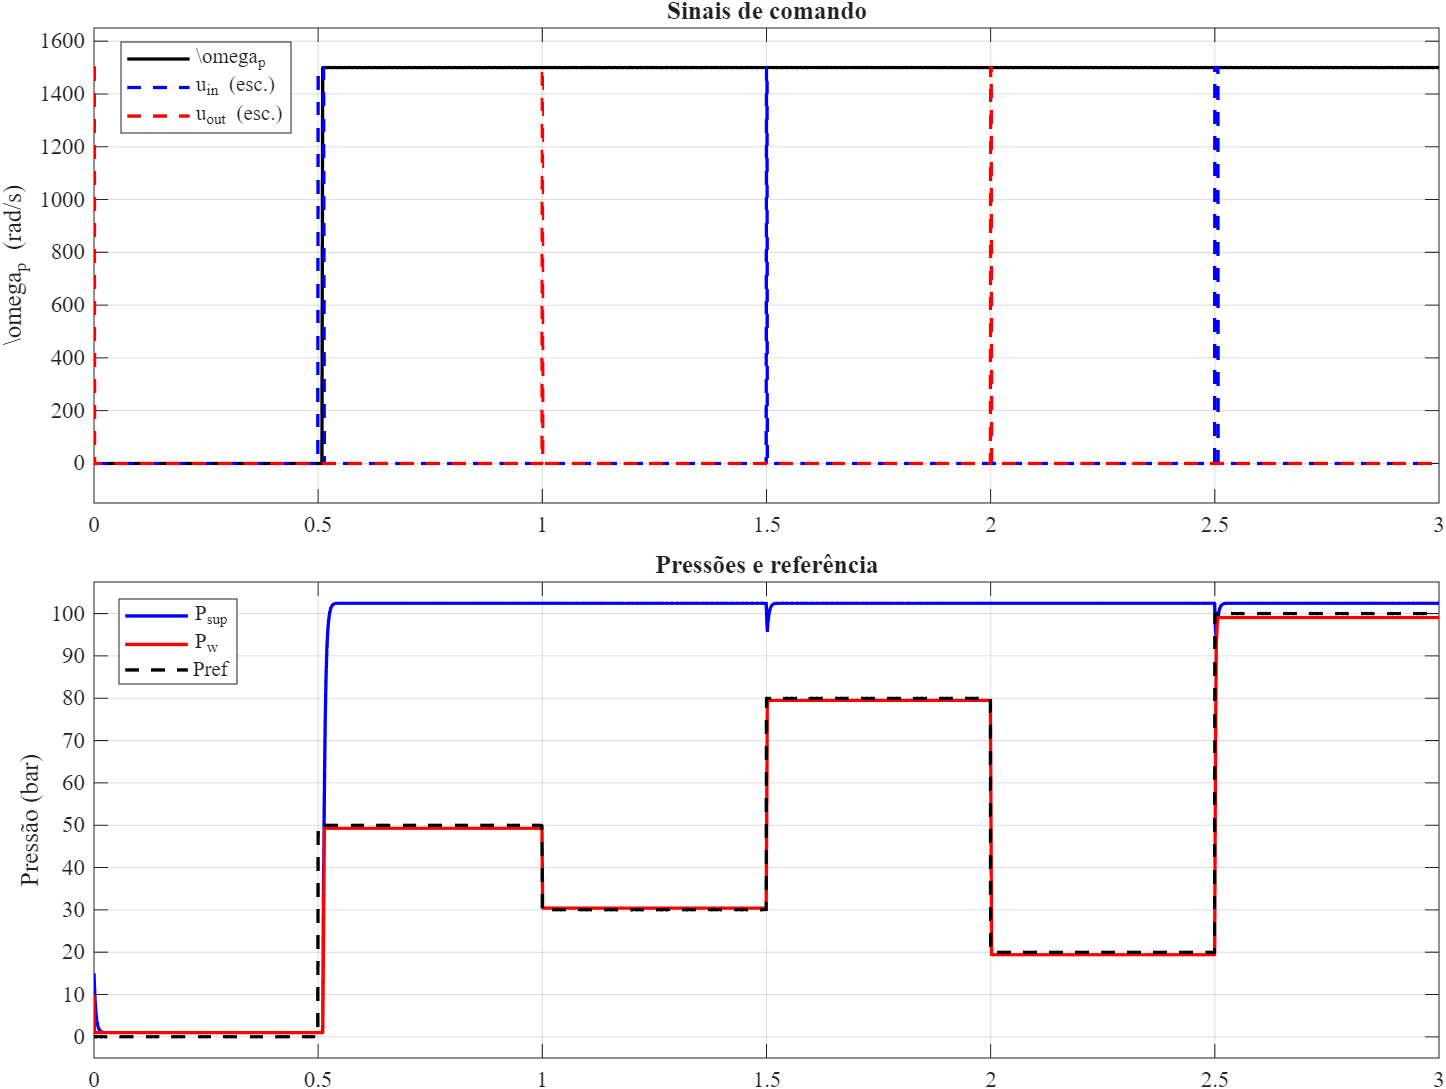
\includegraphics[width=0.95\textwidth]{figuras/simulacao_comandos_e_pressao.png}%
    }{%
        \fbox{\parbox{0.95\textwidth}{\centering Figura a inserir: \texttt{figuras/simulacao\_comandos\_e\_pressao.png}}}%
    }
    \fonte{O Autor.}
\end{figure}

%####################################################################
%####################################################################
%####################################################################
%####################################################################
\subsection{Influência das Saturações}
\label{sec:influencia-saturacoes}

As saturações introduzem uma não linearidade do tipo função limite

\begin{equation}
u_{sat} = \mathrm{sat}(u),
\end{equation}

que modifica a estrutura do sistema em malha fechada.

Quando a ação integral força o crescimento de $u$ além do limite físico, o sistema passa a operar em regime saturado, no qual a dinâmica efetiva deixa de corresponder ao modelo linear utilizado no projeto.

Durante as simulações iniciais, observou-se que limites restritivos nas saturações das pressões e da rotação da bomba impediam o seguimento adequado da referência.

Após ajuste para

\begin{align}
P_{sup}^{\max} &= 2.5 \times 10^{7} \text{ Pa}, \\
P_{w}^{\max} &= 1.5 \times 10^{7} \text{ Pa}, \\
\omega_p^{\max} &= 1500 \text{ rad/s},
\end{align}

o sistema passou a apresentar comportamento coerente com a dinâmica física esperada.

Esse resultado evidencia que restrições artificiais podem comprometer o desempenho do controlador, mesmo quando o projeto teórico é adequado.

%####################################################################
%####################################################################
%####################################################################
%####################################################################
\subsection{Interpretação Física das Limitações Energéticas}
\label{sec:interpretacao-limitacoes-energeticas}

A pressão de alimentação $P_{sup}$ apresentou crescimento significativo durante transientes de carga. Esse comportamento está associado à necessidade de armazenar energia hidráulica suficiente para sustentar a pressão na câmara de roda.

A ação integral contribui para elevar a rotação da bomba enquanto houver erro acumulado, o que pode resultar em aumento temporário de $P_{sup}$. Desde que respeitados os limites físicos do sistema, tal comportamento é coerente com a dinâmica energética do modelo.

%####################################################################
%####################################################################
%####################################################################
%####################################################################
\subsection{Avaliação Quantitativa de Desempenho}
\label{sec:avaliacao-quantitativa-desempenho}

Para complementar a análise qualitativa, foram consideradas métricas quantitativas de desempenho extraídas das respostas temporais obtidas em simulação.

O erro quadrático médio (RMS) foi definido como:

\begin{equation}
e_{RMS} = \sqrt{\frac{1}{T} \int_0^T e^2(t)\, dt},
\end{equation}

onde $e(t) = r(t) - y(t)$ representa o erro de rastreamento.

Além disso, foram avaliados:

\begin{itemize}
    \item Tempo de subida ($t_r$), definido como o intervalo necessário para que a resposta atinja pela primeira vez 90\% do valor de regime;
    \item Tempo de acomodação ($t_s$), correspondente ao instante em que a resposta permanece dentro de uma banda de $\pm 2\%$ do valor final;
    \item Sobressinal máximo ($M_p$), calculado como a diferença percentual entre o pico da resposta e o valor de regime.
    \item Erro estacionário ($e_{\infty}$);
    \item Esforço máximo de controle ($\max |\omega_p|$).
\end{itemize}

As simulações indicaram erro estacionário nulo para degraus de referência dentro da faixa operacional analisada, confirmando a efetividade da ação integral. Os tempos de acomodação observados permaneceram compatíveis com os requisitos dinâmicos esperados para sistemas de atuação hidráulica, sem ocorrência de instabilidades ou oscilações sustentadas.

O esforço máximo de controle foi observado durante transições abruptas de referência, permanecendo dentro da capacidade física especificada para a bomba hidráulica.

Esses resultados corroboram a adequação do controlador LQI para o regime local de operação considerado.

%####################################################################
%####################################################################
%####################################################################
%####################################################################
\section{Considerações sobre Robustez e Limitações}
\label{sec:consideracoes-robustez-limitacoes}

O projeto baseia-se em modelo linear obtido por aproximação local. Assim, a estabilidade garantida pelo LQI refere-se ao sistema linearizado.

A estabilidade do sistema não linear em malha fechada pode ser analisada sob a ótica de estabilidade local no sentido de Lyapunov, sendo garantida em uma vizinhança do ponto de equilíbrio desde que as não linearidades sejam suficientemente suaves.

Entretanto, variações paramétricas significativas ou operação distante do ponto de linearização podem degradar o desempenho. Estratégias como \textit{gain scheduling} ou controle não linear poderiam ampliar a região de validade do controlador.

Esses aspectos indicam que extensões futuras podem incluir:

\begin{itemize}
    \item Estratégias de \textit{anti-windup};
    \item Controle robusto considerando incertezas paramétricas;
    \item Estratégias de linearização múltipla com \textit{gain scheduling}.
\end{itemize}

%####################################################################
%####################################################################
%####################################################################
%####################################################################
